\documentclass[10pt,nocc]{xrese_report}
\usepackage[utf8]{inputenc}
\usepackage{multirow}
\usepackage{setspace}
\usepackage[hidelinks]{hyperref}
\usepackage{algorithm}
\usepackage{algpseudocode}
\usepackage{amsmath,amssymb,amsfonts}
\usepackage{url}
\usepackage{enumitem}
\usepackage{graphicx}
\usepackage[epsilon,tstt]{backnaur}
\usepackage{subfig}

\algnewcommand{\LineComment}[1]{\Statex \(\triangleright\) #1}

\begin{document}
\frontmatter
\project{Multilingual Parsing}

\reportnum{XRESE/2019/001}

\wp{Work-Package 1: ``Tech Report''}

\title{SIGMA -- Systematic Island Grammar forMation Approach}

\date{Oct 2019}

\author{Isaac Griffith}
\affiliation{eXtended Reality and Empirical Software Engineering Lab\\
Department of Informatics and Computer Science\\
Idaho State University
}

\coverart[width=350pt]{images/xrese_logo.png}

\reporttype{Preliminary Report}

%opening

\maketitle
\tableofcontents
\listoffiguresandtables
\listofalgorithms

\mainmatter

\begin{abstract}
\textbf{Introduction}: Since the introduction of island grammars, they've been successfully used for a variety of tasks. This includes impact analysis, multilingual parsing, source code identification, and other tasks. However, there has been no attempt to automate the generation of island grammars.
\textbf{Objective}: This research considers the development of a method to automate the merging of island grammar components. The goal of this is to facilitate the development of an approach to fully automate the creation of island grammars. The end result of which is the reduction in initial effort and maintenance effort required for island grammar engineering. 
\textbf{Methods}: We developed an automated approach to merge components of a grammar. To evaluate this approach we conducted two experiments, each using a factorial design, of 5 replications each. We randomly selected pairs of grammars three size categories to evaluate the effects of the merging process on the maintenance effort and complexity of the generated grammars. 
\textbf{Results}: We found that in all cases the application of this merging approach reduces the maintenance effort and complexity of the grammars. Furthermore, we decrease the similarity threshold (i.e., reduce the degree of similarity between merged components) the greater the change in maintenance effort and complexity. 
\textbf{Limitations}: The primary limitation of this research is that this approach is currently limited to grammars written in the Antlr4 grammar format. 
\textbf{Conclusions}: This work presents the initial steps towards the automated construction of \textit{island} and \textit{tolerant} grammars. We have shown that this approach to merging grammar components follows suit with the expectations of Island and Tolerant grammars (reduction in maintenance effort and complexity).
\end{abstract}

\chapter{Introduction}

The primary paradigm of software application development has been moving steadily away from the homogenous single language and single technology approach and towards a heterogenous multilingual and multi-technology approach for sometime now [@http://zotero.org/users/1776655/items/B8D2E2AR]. Simultaneosly the use of static and dynamic analysis tools as a standard part of a developer's and organizations toolkit has seen rapid growth. Yet, such tools such as SpotBugs\footnote{\url{https://spotbugs.github.io}}, PMD\footnote{\url{https://pmd.github.io}}, Parasoft dotTEST\footnote{\url{https://www.parasoft.com/products/dottest}}, Pylint\footnote{\url{https://www.pylint.org}}, etc. have been designed with a single language or family of languages in mind. Services and software issue accumulation tools such as SonarQube\footnote{\url{https://www.sonarqube.org}} have shown that there is a need for static and dynamic analysis tools to be capable of crossing the boundaries of languages. The typical design paradigm for such tools involves the inclusion of multiple languages via plugins (or some other technique) which requires the use of one or more (language specific) parsers to extract knowledge from the code. Unfortunately, this causes two main issues: 1.) A maintenance nightmare for the inclusion and integration of multiple parsers. 2.) A maintenance headache as languages continue to update and change.

Modern software development practice has led to an increasing number of software systems created using multiple languages. As an example, the modern web application is typically constructed using 5 or more languages (e.g. SQL, Java, TypeScript, HTML, CSS). Such multilingual codebases present a difficult challenge to the development and maintenance of source code analysis tools \cite{mushtaq_multilingual_2017}. Current source analysis tools typically address this challenge using a combination of multiple parsers (one per supported language supported).

Code analysis tools have become an essential part of modern coding [X]. Using these tools, software engineers find bugs, identify security flaws, increase product quality, and comply with business rules and regulations. These tools have been integrated into software build processes and integrated into their pipelines for quality assurance and other services (e.g. SonarQube\texttrademark \footnote{\url{https://sonarqube.org}}).

Island grammars have been shown to be a solution to the problem of developing multilingual parsers \cite{synytskyy_robust_2003}. Though useful, the technique requires the manual combination of selected components from source grammars, a process which can be cumbersome to maintain as these grammars evolve. To overcome this, we propose an automated method to reduce the initial time-consuming manual process and the further difficulty of maintaining the constructed island grammar. In this paper we discuss a key component to the automated construction of island grammars. Specifically, the capability to correctly combine grammar productions together without reducing the grammar's ability to define key aspects of interest.

The automated merging of grammars is an important and necessary step in the evolution of island grammar research. The capability to automate grammar merging addresses the key issues found in the initial construction and further maintenance of island grammars. To evaluate this hypothesis, we used the Goal-Question-Metric (GQM) paradigm \cite{caldiera_goal_1994} to form the following research goal (RG):

\begin{enumerate}[label={\textbf{RG}},left=.2in]
  \item Evaluate an automated approach for the purpose of automating the merging of grammar rules with respect to the maintenance effort and complexity from the point of view of software language engineers in the context of the creation of tolerant and island grammars.
\end{enumerate}

\noindent The solution proposed will allow tool designers to develop source code analysis tools which support multiple programming languages in an efficient and maintainable way.

\section{Organization}

The remainder of this paper is organized as follows. \ref{sec:background} discusses the theoretical foundations and alternative approaches related to this work. \ref{sec:approach} details our approach to automate the merging of grammars which forms the foundation of an initial approach to automating the creation of multilingual parsers, which we call SIGMA. \ref{sec:experimental_design} details the design of experiments which evaluate the proposed approach and its parameterization. \ref{sec:results} presents the results of the experiments. \ref{sec:discussion} presents a discussion of the results and their interpretation in light of other studies. \ref{sec:threats} details the threats to the validity of this study. Finally, this paper is concluded in \ref{sec:conclusions}.

\chapter{Background}

\section{Theoretical Foundations}\label{sec:foundations}

\subsection{Grammars}

A context free grammar, $G$, can be described as \(G = (V,\Sigma{},P,S)\) \cite{haoxiang_languages_1988}. Where, \(V\) is the set of non-terminal symbols, \(\Sigma\) is the set of terminal symbols, \(P \subseteq V \times (V\cup\Sigma)^* \) is the set of productions describing how the symbols of \(V\) can be substituted for other symbols, and \(S \in V\) is the starting symbol. Each production is written as \(a \rightarrow b\) with \(a \in V\) and \(b \in (V\cup\Sigma)^* \). When \(b\) is the empty string, the production is denoted by \(a \rightarrow \varepsilon\). A string, $s$, is called a \textit{valid sentence} for a grammar if it can be created by repeated application of the productions of that grammar \cite{moonen_generating_2001}. \(L(G)\) denotes the set of all valid sentences, or language, of grammar \(G\).

Island Grammars are a specialized form of context free grammar which include the addition of a set of interests. These interests are used to focus the grammar on the set of language components most of interest to the grammar developers. An island grammar is formally defined as the following tuple \(G' = (V,\Sigma{},P,S, I)\) \cite{moonen_generating_2001}. Where, $I$ is the set of interests. These interests, as noted, define the components to which the grammar is focused, these are also known as islands. The remaining components of a language are reduced down into one or more catchall productions referred to as water \cite{moonen_generating_2001}. This has the effect of reducing the complexity of the grammar. An island grammar, $G'$, derived from a grammar, $G$, has a language $L(G')$ which satisfies the following property: \(L(G') \supset L(G)\). Island grammars offer several advantages over regular grammars for many applications including faster development time, lower complexity, and better error tolerance. Due to this island grammars have been used for many applications including documentation extraction and processing \cite{deursen_building_1999}, impact analysis \cite{moonen_lightweight_2002}, and extracting code embedded in natural language documents \cite{bettenburg_what_2008,bacchelli_extracting_2011}. Of particular interest to our research is their use for creating multilingual parsers \cite{synytskyy_robust_2003}, which inspired this research, and research into the development of tolerant grammars \cite{klusener_deriving_2003,goloveshkin_tolerant_2018,kurs_bounded_2015}.

\subsection{Grammar Metrics}

\section{Alternative Approaches}\label{sec:related}

Using an intermediate representation (IR), such as Java\texttrademark\ bytecode or Microsoft IL, is a common method for performing operations on multilingual code bases. This allows code analysis tools to be built around the language(s) defined by the IR rather than having to deal with each of the different languages individually. However, using an IR doesn't work when analyzing systems created from languages that do not share a common IR [X]. Using an IR also doesn't work if performing manipulations of source code or if there isn't a clear correspondence between a source language and its IR. An example of this can be seen for PIT \cite{coles_pit:_2016}, a Java mutation testing framework. Even though their system is designed around transforming and manipulating java bytecode, the system struggles with handling bytecode generated by other JVM languages. However, they still have had limited success with other JVM languages.

Another approach that's been developed for analyzing multilingual systems is through the use of a separate parser for each language [A-Z]. Constructing and integrating each parser for each language can be both difficult and time consuming, and thus it is better to use existing parsers \cite{petrinja_how_2013}. Using existing parsers, one can modify the abstract syntax trees into a language independent form [X]. The problem one contends with in this approach is these parsers may be written in a variety of languages. The use of an existing Island Grammar\cite{synytskyy_robust_2003} may alleviate these issues, but typically they tend to be specific to their particular problem and their construction is currently a time-consuming manual process.

\section{Research Contributions}

In this paper we develop the following contributions:

\begin{enumerate}
 \item The proposal of an algorithmic approach to the generation of island grammars from multiple grammars.
 \item Case study results concerning island grammar generation and grammar measurement.
 \item A tool which provides the capability to automate the proposed processes.
\end{enumerate}

\chapter{Algorithms}

\section{Normalization Algorithm}\label{sec:norm_alg}

The following algorithm defines the approach for normalizing a given grammar. The normalization process defined here facilitates the ability to merge productions, in pursuit of the overarching goal of automated generation of Island [X], Tolerant [X], Bridge [X], and Bounded Seas [X] grammars.

This algorithm assumes that the source grammar, $G$, was initially in some defined formalism such as Antlr [X], EBNF [X], BNF [X], SDF [X], TXL [X], etc. The grammar was then read in and processed to conform to the metamodel depicted in Figure \ref{fig:metamodel}. Assuming that the grammar meets this condition, the goal of this algorithm is then to reformat the grammar such that each production is of one of the following forms:

\begin{figure}
 \begin{center}
  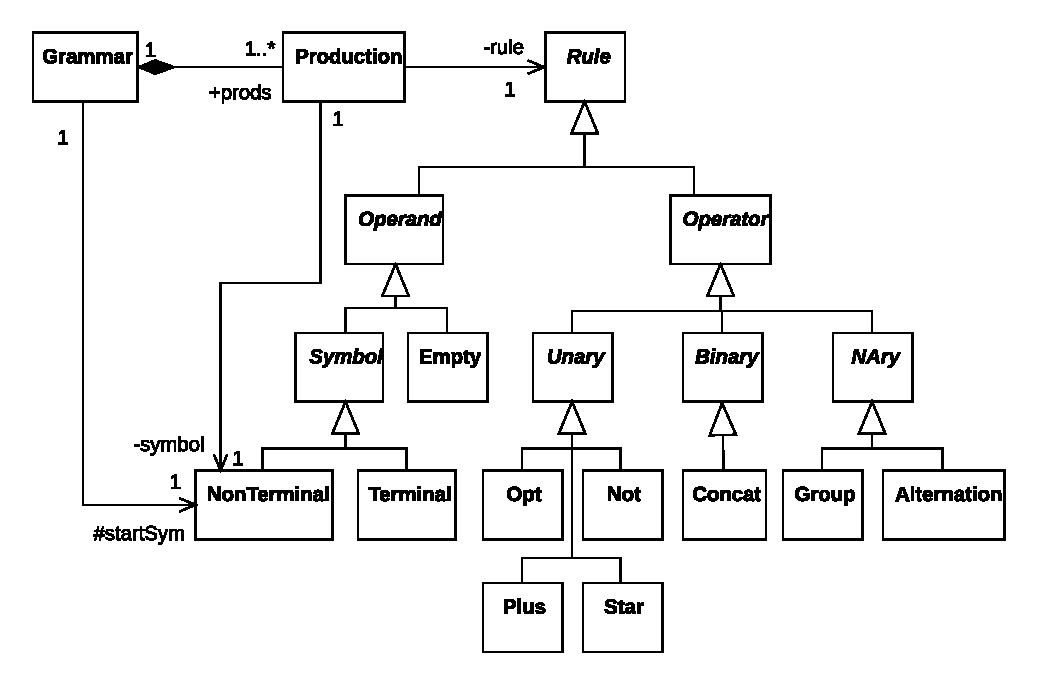
\includegraphics[width=\textwidth]{images/paper/metamodel.eps}
  \caption{Grammar metamodel.}\label{fig:metamodel}
 \end{center}
\end{figure}


\begin{itemize}
 \item \textit{Form\textsubscript{1}}: A production composed of a rule containing at least one symbol, and where all symbols are concatenated with one another. An example is: $\left<A\right> ::= \left<B\right> \textrm{`a'} \ldots$.
 \item \textit{Form\textsubscript{2}}: A production composed of an alternation of one or more symbols. An example is: $\left<B\right> ::= \left<A\right>\,|\,\textrm{`b'}\,|\,\ldots\,|\,\varepsilon$.
\end{itemize}

\begin{algorithm}[tb]
 \caption{Normalization Algorithm}\label{alg:norm}
 
 \begin{algorithmic}[1]
  \Procedure{Normalize}{$\mathcal{G}$}
   \Repeat
     \State $\mathcal{G} \gets$ \Call{EliminateUnusedProductions}{$\mathcal{G}$}
     \State $\mathcal{G} \gets$ \Call{SimplifyProductions}{$\mathcal{G}$}
     \State $\mathcal{G} \gets$ \Call{MergeEquivProductions}{$\mathcal{G}$}
     \State $\mathcal{G} \gets$ \Call{EliminateUnitProductions}{$\mathcal{G}$}
     \State $\mathcal{G} \gets$ \Call{ExpandProductions}{$\mathcal{G}$}
     \State $\mathcal{G} \gets$ \Call{CollapseProductions}{$\mathcal{G}$}
   \Until{\Call{Unchanged}{$\mathcal{G}$}}
  \EndProcedure
 \end{algorithmic}
\end{algorithm}

The normalization process, as defined in Algorithm \ref{alg:norm}, repeatedly executes six processes until the grammar stabilizes. These six processes are: i) eliminating unused rules, ii) simplifying productions, iii) merging equivalent rules, iv) eliminating unit rules, v) expanding productions, and vi) collapsing compatible productions.

\subsection{Eliminating Unused Rules}

This process removes all productions that are not produced, directly or indirectly, from the start production. This is accomplished by marking all productions enumerated via a depth first search (see Algorithm \ref{alg:dfsmark}), and then dropping unmarked productions, as shown in Algorithm \ref{alg:elim_unused_prod}. When applied to $G_3$ the grammar is transformed into grammar $G_4$, as depicted in Figure \ref{fig:grammar_g4}.

\begin{algorithm}[tb]
\caption{Eliminate Unused Productions}\label{alg:elim_unused_prod}
 \begin{algorithmic}[1]
  \Function{EliminateUnusedProductions}{$\mathcal{G}$}
    \State $H \gets (V,E)$ \LineComment Create empty graph
    \ForAll{$p \in \mathcal{G}.\Sigma$}
      \State $\mathcal{H}.V \gets \mathcal{H}.V \cup \{p\}$
    \EndFor
    \ForAll{$p \in \mathcal{G}.\Sigma$}
      \ForAll{$nt \in p.rule$} \LineComment Create directed edge between non-terminals
        \State $\mathcal{H}.E \gets \mathcal{H}.E \cup \{(p, nt)\}$
      \EndFor
    \EndFor
    \State \Call{DFSMark}{$\mathcal{G}.S$}
    \ForAll{$v \in {H}.V$}
      \If{$!$\Call{isMarked}{$v$}}
        \State $\mathcal{G}.\Sigma \gets \mathcal{G}.\Sigma - \{v.value\}$
      \EndIf
    \EndFor
  \EndFunction
 \end{algorithmic}
\end{algorithm}

\begin{algorithm}[tb]
\caption{Depth First Marking}\label{alg:dfsmark}
 \begin{algorithmic}[1]
  \Function{DFSMark}{$start$}
    \State $\mathcal{S} \gets [start]$
    \While{$\mathcal{S} \ne \varnothing$}
      \State $p \gets$ \Call{pop}{$\mathcal{S}$}
      \State \Call{Mark}{$p$}
      \ForAll{$s \in $\Call{succ}{$p$}}
        \If{$!$\Call{isMarked}{$s$}}
          \State \Call{push}{$\mathcal{S},s$}
        \EndIf
      \EndFor
    \EndWhile
  \EndFunction
 \end{algorithmic}
\end{algorithm}

\begin{figure}[tb]
 \centering
 \subfloat[Grammar $G_4$.]{
   \label{fig:grammar_g4}
   \begin{minipage}[t]{.4\textwidth}
\begin{bnf*}
\bnfprod{S}{\bnfpn{\(S_1\)} \bnfor \bnfpn{\(S_2\)}}\\
\bnfprod{$S_1$}{\bnfpn{A} \bnfor \bnfpn{B}}\\
\bnfprod{A}{\bnfts{a} \bnfsp \bnfes \bnfsp \bnfpn{B} \bnfsp \bnfpn{\(C_1\)}}\\
\bnfprod{$C_1$}{\bnfts{c}}\\
\bnfprod{B}{\bnfts{b} \bnfsp \bnfts{d}}\\
\bnfprod{$S_2$}{\bnfpn{\(C_2\)} \bnfor \bnfpn{D}}\\
\bnfprod{$C_2$}{\bnfts{c}}\\
\bnfprod{D}{\bnfts{a} \bnfsp \bnfts{d} \bnfsp (\bnfts{e} \bnfor \bnfts{c}) \bnfor (\bnfpn{\(C_2\)} \bnfor \bnfts{b})}
\end{bnf*}
 \end{minipage}
}
 \qquad
 \subfloat[Grammar $G_5$.]{
   \label{fig:grammar_g5}
   \begin{minipage}[t]{.4\textwidth}
\begin{bnf*}
\bnfprod{S}{\bnfpn{\(S_1\)} \bnfor \bnfpn{\(S_2\)}}\\
\bnfprod{$S_1$}{\bnfpn{A} \bnfor \bnfpn{B}}\\
\bnfprod{A}{\bnfts{a} \bnfsp \bnfpn{B} \bnfsp \bnfpn{\(C_1\)}}\\
\bnfprod{$C_1$}{\bnfts{c}}\\
\bnfprod{B}{\bnfts{b} \bnfsp \bnfts{d}}\\
\bnfprod{$S_2$}{\bnfpn{\(C_2\)} \bnfor \bnfpn{D}}\\
\bnfprod{$C_2$}{\bnfts{c}}\\
\bnfprod{D}{\bnfts{a} \bnfsp \bnfts{d} \bnfsp (\bnfts{e} \bnfor \bnfts{c}) \bnfor (\bnfpn{\(C_2\)} \bnfor \bnfts{b})}
\end{bnf*}
 \end{minipage}
}
 \qquad
 \subfloat[Grammar $G_6$.]{
   \label{fig:grammar_g6}
   \begin{minipage}[t]{.4\textwidth}
\begin{bnf*}
\bnfprod{S}{\bnfpn{\(S_1\)} \bnfor \bnfpn{\(S_2\)}}\\
\bnfprod{$S_1$}{\bnfpn{A} \bnfor \bnfpn{B}}\\
\bnfprod{A}{\bnfts{a} \bnfsp \bnfpn{B} \bnfsp \bnfpn{C}}\\
\bnfprod{C}{\bnfts{c}}\\
\bnfprod{B}{\bnfts{b} \bnfsp \bnfts{d}}\\
\bnfprod{$S_2$}{\bnfpn{C} \bnfor \bnfpn{D}}\\
\bnfprod{D}{\bnfts{a} \bnfsp \bnfts{d} \bnfsp (\bnfts{e} \bnfor \bnfts{c}) \bnfor (\bnfpn{C} \bnfor \bnfts{b})}
\end{bnf*}
 \end{minipage}
}
 \qquad
 \subfloat[Grammar $G_7$.]{
   \label{fig:grammar_g7}
   \begin{minipage}[t]{.4\textwidth}
\begin{bnf*}
\bnfprod{S}{\bnfpn{\(S_1\)} \bnfor \bnfpn{\(S_2\)}}\\
\bnfprod{$S_1$}{\bnfpn{A} \bnfor \bnfpn{B}}\\
\bnfprod{A}{\bnfts{a} \bnfsp \bnfpn{B} \bnfsp \bnfts{c}}\\
\bnfprod{B}{\bnfts{b} \bnfsp \bnfts{d}}\\
\bnfprod{$S_2$}{\bnfts{c} \bnfor \bnfpn{D}}\\
\bnfprod{D}{\bnfts{a} \bnfsp \bnfts{d} \bnfsp (\bnfts{e} \bnfor \bnfts{c}) \bnfor (\bnfts{c} \bnfor \bnfts{b})}
\end{bnf*}
 \end{minipage}
}
 \qquad
 \subfloat[Grammar $G_8$.]{
   \label{fig:grammar_g8}
   \begin{minipage}[t]{.3\textwidth}
\begin{bnf*}
\bnfprod{S}{\bnfpn{\(S_1\)} \bnfor \bnfpn{\(S_2\)}}\\
\bnfprod{$S_1$}{\bnfpn{A} \bnfor \bnfpn{B}}\\
\bnfprod{A}{\bnfts{a} \bnfsp \bnfpn{B} \bnfsp \bnfts{c}}\\
\bnfprod{B}{\bnfts{b} \bnfsp \bnfts{d}}\\
\bnfprod{$S_2$}{\bnfts{c} \bnfor \bnfpn{D}}\\
\bnfprod{D}{\bnfpn{\(D_1\)} \bnfor \bnfpn{\(D_3\)}}\\
\bnfprod{\(D_1\)}{\bnfts{a} \bnfsp \bnfts{d} \bnfsp \bnfpn{\(D_2\)}}\\
\bnfprod{\(D_2\)}{\bnfts{e} \bnfor \bnfts{c}}\\
\bnfprod{\(D_3\)}{\bnfts{c} \bnfor \bnfts{b}}
\end{bnf*}
 \end{minipage}
}
 \qquad
 \subfloat[Grammar $G_9$.]{
   \label{fig:grammar_g9}
   \begin{minipage}[t]{.3\textwidth}
\begin{bnf*}
\bnfprod{S}{\bnfpn{A} \bnfor \bnfpn{B} \bnfor \bnfts{c} \bnfor \bnfpn{D}}\\
\bnfprod{A}{\bnfts{a} \bnfsp \bnfts{b} \bnfsp \bnfts{d} \bnfsp \bnfts{c}}\\
\bnfprod{B}{\bnfts{b} \bnfsp \bnfts{d}}\\
\bnfprod{D}{\bnfpn{\(D_1\)} \bnfor \bnfts{c} \bnfor \bnfts{b}}\\
\bnfprod{\(D_1\)}{\bnfts{a} \bnfsp \bnfts{d} \bnfsp \bnfpn{\(D_2\)}}\\
\bnfprod{\(D_2\)}{\bnfts{e} \bnfor \bnfts{c}}
\end{bnf*}

 \end{minipage}
 }
 \caption{Transformed grammars produced during the normalization of grammar $G_3$.}
\end{figure}

\subsection{Simplifying Productions}

This process aims to simplify productions. This is achieved by first removing $\varepsilon$'s embedded inside rules. Once this is complete productions containing a single term are replaced with that term. This process is embodied in Algorithm \ref{alg:simp_prod}. When to grammar $G_4$, it is transformed into grammar $G_5$, as depicted in \ref{fig:grammar_g5}.

\begin{algorithm}[tb]
\caption{Simplify Productions}\label{alg:simp_prod}
 \begin{algorithmic}[1]
  \Function{SimplifyProductions}{$\mathcal{G}$}
    \LineComment Remove embedded $\varepsilon$'s
    \ForAll{$p \in \mathcal{G}.\Sigma$}
      \If{\Call{contains}{$p,concat(\varepsilon)$}}
        \State \Call{remove}{$p,\varepsilon$}
      \EndIf
    \EndFor
    \LineComment Replace one-term productions
    \ForAll{$p \in \mathcal{G}.\Sigma$}
      \If{$|p.rule| = 1$}
        \State \Call{replace}{$uses(p),p.rule$}
      \EndIf
    \EndFor
  \EndFunction
 \end{algorithmic}
\end{algorithm}

\subsection{Merging Equivalent Productions}

Productions that have identical rules are replaced by a single production. This new production is given a name derived from the productions that were merged to create it. In the following example of this step, rules a and b are merged into the rule a+b:

\begin{bnf*}
\bnfprod{s}{\bnfpn{a} \bnfor \bnfpn{b}}\\
\bnfprod{a}{\bnfts{a} \bnfsp \bnfts{b} \bnfsp \bnfpn{a}}\\
\bnfprod{b}{\bnfts{a} \bnfsp \bnfts{b} \bnfsp \bnfpn{a}}
\end{bnf*}

\noindent Which after equivalent rules are merged yields:

\begin{bnf*}
\bnfprod{s}{\bnfpn{a+b}}\\
\bnfprod{a+b}{\bnfts{a} \bnfsp \bnfts{b} \bnfsp \bnfpn{a+b}}
\end{bnf*}

\noindent When this step is applied to grammar $G_5$, it is transformed into grammar $G_6$, as depicted in Figure \ref{fig:grammar_g6}.

\begin{algorithm}[tb]
\caption{Merge Equivalent Productions}\label{alg:merge_equiv_prod}
 \begin{algorithmic}[1]
  \Function{MergeEquivProductions}{$\mathcal{G}$}
    \State $pairs \gets \varnothing$
    \For{$i \in [0,|\mathcal{G}.\Sigma|)$}
      \For{$j \in (i, |\mathcal{G}.\Sigma|)$}
        \If{$i \ne j$}
          \State $pairs \gets pairs \cup (\mathcal{G}.\Sigma[i], \mathcal{G}.\Sigma[j])$
        \EndIf
      \EndFor
    \EndFor
    \ForAll{$p \in pairs$}
      \If{$p.left.rule = p.right.rule$}
        \State \Call{CombineAndReplace}{$p.left,p.right$}
      \EndIf
    \EndFor
  \EndFunction
 \end{algorithmic}
\end{algorithm}

\subsection{Eliminating Unit Productions}

All non-terminals with productions of one of the following two forms will have their non-terminal symbols replaced by their rules, and their productions eliminated.

\begin{bnf*}
\bnfprod{a}{\bnfpn{b}}\\
\bnfprod{a}{\bnfts{a}}
\end{bnf*}

\noindent Elimination of productions of the first form, is derived from Chomsky Normal Form (CNF) [X]. Eliminations of productions of the second form, a derivation from CNF, allows the simplification process to simplify rules of the following form:

\begin{bnf*}
\bnfprod{a}{\bnfpn{b} \bnfsp \bnfts{a} \bnfsp \bnfts{b}}\\
\bnfprod{b}{\bnfes}
\end{bnf*}

\noindent When this step is applied to grammar $G_6$, it is transformed into grammar $G_7$, as depicted in Figure \ref{fig:grammar_g7}.

\begin{algorithm}[tb]
\caption{Eliminate Unit Productions}\label{alg:elim_unit_prod}
 \begin{algorithmic}[1]
  \Function{EliminateUnitProductions}{$\mathcal{G}$}
    \ForAll{$p \in \mathcal{G}.\Sigma$}
      \If{$|p.rule| = 1$}
        \State \Call{replace}{$uses(p),p.rule$}
      \EndIf
    \EndFor
  \EndFunction
 \end{algorithmic}
\end{algorithm}

\subsection{Expanding Productions}

Productions that have nested rules have all nested content replaced by with a non-terminal. The new non-terminal defines a production pointing to their content. When this step is applied to grammar $G_7$, it is transformed into grammar $G_8$, as depicted in Figure \ref{fig:grammar_g8}.

\begin{algorithm}[tb]
\caption{Expand Productions}\label{alg:expand_prod}
 \begin{algorithmic}[1]
  \Function{ExpandProductions}{$\mathcal{G}$}
    \Repeat
      \State $changed \gets \bot$
      \ForAll{$p \in \mathcal{G}.\Sigma$}
        \If{\Call{isConcat}{$p.rule$}}
          \ForAll{$g \in p.rule$}
            \If{\Call{isGroup}{$g$}}
              \State \Call{createAndReplaceWithProd}{$g$}
              \State $changed \gets \top$
            \EndIf
          \EndFor
        \ElsIf{\Call{isAlt}{$p.rule$}}
          \ForAll{$a \in p.rule$}
            \State \Call{createAndReplaceWithProd}{$a$}
            \State $changed \gets \top$
          \EndFor
        \EndIf
      \EndFor
    \Until{$changed = \bot$}
  \EndFunction
 \end{algorithmic}
\end{algorithm}

\subsection{Collapsing Compatible Productions}

The final step of the normalization process combines productions that are compatible with each other. This ensures that any non-terminal symbols referenced in a rule will not define a duplicate production. The following provides an example:

\begin{bnf*}
\bnfprod{A}{\bnfts{a} \bnfsp \bnfpn{B}}\\
\bnfprod{B}{\bnfts{b} \bnfsp \bnfts{c}}\\
\bnfprod{C}{\bnfts{c} \bnfor \bnfpn{D}}\\
\bnfprod{D}{\bnfts{d} \bnfor \bnfts{e}}
\end{bnf*}

\noindent would then collapse to form:

\begin{bnf*}
\bnfprod{A}{\bnfts{a} \bnfsp \bnfts{b} \bnfsp \bnfts{c}}\\
\bnfprod{C}{\bnfts{c} \bnfor \bnfts{d} \bnfor \bnfts{e}}
\end{bnf*}


\noindent When this step is applied to grammar $G_8$, it is transformed into grammar $G_9$, as depicted in Figure \ref{fig:grammar_g9}.

\begin{algorithm}[tb]
\caption{Collapse Productions}\label{alg:coll_prod}
 \begin{algorithmic}[1]
  \Function{CollapseProductions}{$\mathcal{G}$}
    \LineComment Split productions into form1 and form2
    \State $f_1 \gets$ \Call{Collect}{``form1''}
    \State $f_2 \gets$ \Call{Collect}{``form2''}
    \ForAll{$p \in f_1$}
      \If{\Call{OnlyTerminals}{$p.rule$}}
        \State \Call{ReplaceF1UsesWithRule}{$p$}
      \EndIf
    \EndFor
    \ForAll{$p \in f_2$}
      \If{\Call{OnlyTerminals}{$p.rule$}}
        \State \Call{ReplaceF2UseWithRule}{$p$}
      \EndIf
    \EndFor
  \EndFunction
 \end{algorithmic}

\end{algorithm}


\section{Merging Algorithm}\label{sec:merge_alg}

\begin{algorithm}[tb]
 \caption{Merge Algorithm}\label{alg:merge_prods}
 \begin{algorithmic}[1]
  \Procedure{MergeProductions}{$\mathcal{N}, t$}
    \State $f_1 \gets collect(\textrm{`form1'}, \mathcal{N})$
    \State $f_2 \gets collect(\textrm{`form2'}, \mathcal{N})$
    
    \State $p_1 \gets $ \Call{Pairs}{$f_1$}
    \State $p_2 \gets $ \Call{Pairs}{$f_2$}
    
    \State $\mathcal{Q}_1 \gets$ \Call{Measure}{$p_1,t,S_1$}
    \State $\mathcal{Q}_2 \gets$ \Call{Measure}{$p_2,t,S_2$}
    
    \While{$\mathcal{Q}_1 \ne \varnothing \vee \mathcal{Q}_2 \ne \varnothing$}
      \State \Call{Process}{$\mathcal{Q}_1,f_1,S_1$}
      \State \Call{Process}{$\mathcal{Q}_2,f_2,S_2$}
    \EndWhile
  \EndProcedure
 \end{algorithmic}
\end{algorithm}

\begin{algorithm}[tb]
\caption{Form Pairs}\label{alg:form_pairs}
 \begin{algorithmic}[1]
  \Function{Pairs}{$list$}\Comment $O(n\log n)$
    \State $x \gets 0$
    \For{$i \in [0,length(list))$}
      \For{$j \in (i,length(list))$}
        \State $list[x] \gets (list[i], list[j])$
        \State $x \gets x + 1$
      \EndFor
    \EndFor
  \EndFunction
 \end{algorithmic}
\end{algorithm}

\begin{algorithm}[tb]
\caption{Construct Priority Queues}\label{alg:const_pq}
 \begin{algorithmic}[1]
  \Function{Measure}{$data,t,func$}\Comment $O(n\log n)$
    \State $\mathcal{Q} \gets []$
    \ForAll{$p\in data$}
      \State $s \gets $ \Call{$func$}{$p.a, p.b$}
      \If{$s \geq t$}
        \State \Call{Offer}{$\mathcal{Q}$,$\left< p,t\right>$}
      \EndIf
    \EndFor
    \State \Return $\mathcal{Q}$
  \EndFunction
 \end{algorithmic}
\end{algorithm}

The following algorithms define the approach for merging similar productions of a grammar. This approach assumes that the grammar has been normalized such that each production in the grammar is one of the following two forms:

\begin{itemize}
 \item \textit{Form\textsubscript{1}}: A production composed of a rule containing at least one symbol, and where all symbols are concatenated with one another. An example is: $\left<A\right> ::= \left<B\right> \textrm{`a'} \ldots$.
 \item \textit{Form\textsubscript{2}}: A production composed of an alternation of one or more symbols. An example is: $\left<B\right> ::= \left<A\right>\,|\,\textrm{`b'}\,|\,\ldots\,|\,\varepsilon$.
\end{itemize}

The algorithm initially separates all existing productions of the normalized grammar, $\mathcal{N}$ into two disjoint sets of productions based on the form the productions take. These sets are then used to compose pairs of productions which will be compared for similarity. This process uses a simple nested loop approach (the function \textit{Pairs} in lines 13--21 in Algorithm \ref{alg:merge}). These pairs are then used to form two priority queues (one per form type) via the $Measure$ function in Algorithm \ref{alg:merge}.

\subsection{Measure}

\begin{algorithm}[tb]
\caption{Measures $S_1$ and $S_2$}\label{alg:measures}
 \begin{algorithmic}[1]
  \Function{$S_1$}{$a,b$}
    \State \Return $\frac{2|\textrm{aligned}(a,b)|}{|a| + |b|}$
  \EndFunction
  \Statex
  \Function{$S_2$}{$a,b$}
    \State \Return $\frac{2|a \cap b|}{|a| + |b|}$
  \EndFunction
 \end{algorithmic}

\end{algorithm}

The measure function walks through the list of pairs provided to determine which will be considered during the actual merging process. For each pair of productions, a similarity score is measured, depending on the form. For productions of type \textit{Form\textsubscript{1}} the similarity is measured using equation \ref{eqn:form1}. This equation compares the size of the aligned components of two production rules to the total size of the productions.

\begin{eqnarray}\label{eqn:form1}
 S_1 & = & \frac{2|aligned(A,B)|}{|A| + |B|}
\end{eqnarray}

The function $aligned$ aligns two rules as follows. A data structure composed of two doubly linked lists, whose elements are the symbols of a rule. Items in each list which contain the same symbol are then linked with alignment links. Initially, any alignment link which crosses another is removed. This continues, until no links can be removed. The value used in this equation is then the number of links remaining in the data structure. This value is doubled in order to account for the number of connected nodes rather than edges.

The similarity of productions of type \text{Form\textsubscript{2}} are measured using Equation \ref{eqn:form2}. In this equation we simply calculate the size of the intersection of symbols of each production divided by the total number of symbols in both productions. We again double the numerator to account for the use of common symbols in both productions.

\begin{eqnarray}\label{eqn:form2}
 S_2 & = & \frac{2|A \cap B|}{|A| + |B|}
\end{eqnarray}


Finally, in either case we compare the similarity of the two productions to a known threshold value, $t$. If the value is less than the threshold, we disregard the pair, else we offer it to a priority queue (which is sorted on similarity). The priority queues will be utilized during the merging process.

\subsection{Process}

\begin{algorithm}[tb]
\caption{Process Productions}\label{alg:process}
 \begin{algorithmic}[1]
  \Function{Process}{$\mathcal{Q},data,func$}
    \While{$\mathcal{Q} \ne \varnothing$}
      \State $p \gets$ \Call{Poll}{$\mathcal{Q}$}
      \State $\mathcal{V} \gets$ \Call{Merge}{$p.pair$}
      \State $\mathcal{Q} \gets$ \Call{Update}{$\mathcal{Q},\mathcal{V},p,data,func$}
    \EndWhile
  \EndFunction
 \end{algorithmic}
\end{algorithm}

The process function, shown in Algorithm \ref{alg:process}, processes a priority queue of pairs of productions. The priority queue is sorted on the similarity between the two productions to be merged. The most similar pair is initially polled from the queue and then merged to form a new set of normalized productions. These normalized productions are then used to update the queue based on the provided similarity scoring function. This process continues until the priority queue is empty.

\subsection{Merge}

\begin{algorithm}[tb]
 \caption{Merge Algorithm}\label{alg:merge}
 \begin{algorithmic}[1]
  \Function{Merge}{$pair$}
    \If{$pair$ is of form1}
      \State $list \gets$ \Call{createAlignmentList}{$pair$}
      \ForAll{$e \in list.alignments$}
        \If{\Call{isCrossing}{$e$}}
          \State \Call{delete}{$e$}
        \EndIf
      \EndFor
      \Repeat
        \State $changed \gets \bot$
        \ForAll{$e \in list.alignments$}
          \If{$e.left > e.right$}
            \State \Call{Insert}{$list.right,\varepsilon,e.right$}
            \State $changed \gets \top$
          \ElsIf{$e.left < e.right$}
            \State \Call{Insert}{$list.left,\varepsilon,e.left$}
            \State $changed \gets \top$
          \EndIf
        \EndFor
      \Until{$changed = \bot$}
      \ForAll{$p\in list$}
        \If{$p.left = p.right$}
          \State $rule \gets rule \cdot p.left$
        \ElsIf{$p.left = \varepsilon$}
          \State $rule \gets rule \cdot (p.right | p.left)$
        \Else
          \State $rule \gets rule \cdot (p.left | p.right)$
        \EndIf
      \EndFor
    \Else
      \State $v \gets \varnothing$
      \State $v.symbol \gets a.symbol + \textrm{' '} + b.symbol$
      \State $v.rule \gets a.rule \cup b.rule$
    \EndIf
    \State $\mathcal{V} \gets$ \Call{Normalize}{$v$}
    \State \Return{$\mathcal{V}$}
  \EndFunction  
 \end{algorithmic}

\end{algorithm}

The merge function, shown in Algorithm \ref{alg:merge}, is where the actual merging of productions occurs. This process is dependent on whether the pair of productions to be merged are of $Form_1$ or $Form_2$. In the former case, an alignment list data structure is created containing the symbols from each production. This data structure is two parallel linked lists (used to maintain the order of the original symbols). The elements in common between the two lists are then linked by what are called ``alignment edges''. These edges form a bipartite graph between the nodes of the lists.

Alignment edges are then processed to determine if they cross any other edges. This is determined by comparing edges with the largest difference in list indexes against all other edges. If it is determined that a crossing has occurred, the largest difference edge is removed. At this point only edges which can be aligned will remain and the alignment process begins.

The alignment process works as follows. For each edge, starting with the edge with the smallest index (on one side), if the indexes on both sides of the list are not equal, an empty string node is inserted into the list with the node of lesser index. This process continues until all edges are aligned. Once all edges are aligned, pairs are formed by combining the nodes from both lists at the same index. If the nodes contain different symbols, they are grouped by alternation and then concatenated to the rule.

In the case of $Form_2$ productions. The pair is merged by the union of symbols between the two productions. This forms an alternation between each of the symbols in the union.

In both cases, once the merge is completed the new production is then normalized (which may produce multiple new productions in the case of $Form_1$ productions). This set of productions is then returned.

\subsection{Update}

\begin{algorithm}[tb]
 \caption{Update Algorithm}\label{alg:update}
 \begin{algorithmic}[1]
  \Function{Update}{$\mathcal{Q},v,p,data,func$}\Comment $O(n\log n)$
    \State $data \gets data - \{p.a,p.b\}$
    \ForAll{$i \in \mathcal{Q}$}
      \If{$contains(i,p.a) \vee contains(i,p.b)$}
        \State \Call{Remove}{$\mathcal{Q},i$}
      \EndIf
    \EndFor
    \ForAll{$d \in data$}
      \State $s \gets$ \Call{$func$}{$v,d$}
      \If{$s \geq t$}
        \State \Call{Offer}{$\mathcal{Q},\left<d,v\right>$}
      \EndIf
    \EndFor
    \State $data \gets data \cup \{v\}$
    \ForAll{$p \in \mathcal{N}$}
      \If{\Call{Contains}{$p,a$}}
        \State \Call{ReplaceAndNormalize}{$p,a,v$}
      \ElsIf{\Call{Contains}{$p,b$}}
        \State \Call{ReplaceAndNormalize}{$p,b,v$}
      \EndIf
    \EndFor
  \EndFunction
 \end{algorithmic}
\end{algorithm}

Finally, once a pair of productions have been merged and their result normalized the priority queue and grammar must be updated to account for the change. The process for this is defined by the Update function shown in Algorithm \ref{alg:update}. Initially, the data set containing the pair of merged productions is updated by removing the pair. Then the priority queue is updated by identifying all pairs in the queue which contain either of the pair that was merged and if found such pairs are removed from the queue. The grammar is updated to replace all uses of the merged productions are replaced with the newly created merged production. Finally, Using the remaining set of productions of the same form as the merged production, the new productions are then paired with all remaining productions in the set and the similarity between pairs is measured. If the similarity is above the similarity threshold, then the pair is added to the priority queue.

\subsection{Outcome}

The outcome of this algorithm is that those productions with a similarity of at least $t$ are combined into single productions, and then re-normalized to one of the two forms noted at the beginning of Section \ref{sec:merge_alg}. It is plain to see that the mechanics of this process will ensure that for a normalized grammar, $G$ for some language $L_G$, that the resulting grammar, $G'$, will produce a language $L_{G'} \supseteq L_{G}$. This is due to the fact that in the case of \textit{Form\textsubscript{1}} merges the order of the symbols is maintained, and for those symbols which cannot be paired an alternation with the empty string is injected. This is equivalent to constructing an optional symbol in EBNF which relaxes the resulting grammar, but which also maintains the capability of the previous grammar.

In the case of \textit{Form\textsubscript{2}} productions, it is plain to see that the merging maintains a similar property as well. In this case both productions are simply an alternation of one or more productions and hence the union of two alternations will relax the resulting grammar, but maintains the capabilities of the source grammar.

\section{Islandization}

This section describes the methods we have developed to automate the generation of multilingual island grammars. In the following subsections we detail the algorithms we have designed to complete this task. We then describe the operation of these algorithms on simple grammars. Finally, we detail the design of the tool which implements these algorithms and provides a platform to facilitate data collection associated with experimentation with these algorithms.

\begin{algorithm}
 \caption{Islandization}
 \begin{algorithmic}[1]
  \Procedure{Islandization}{$G,I$}
    \LineComment for each interest item in I mark corresponding productions in G as interest
    \ForAll{$i \in I$}
      \State $p \gets$ \Call{findProduction}{$G,i$}
      \State \Call{markAsInterest}{$p$}
    \EndFor
    \LineComment Create fresh Start Production, Water Production, and Island Production in new grammar G'
    \State $S \gets (W\,|\,I)$
    \State $G' \gets (V,\Sigma,P,S)$
    \LineComment{Construct Island Production I}
    \ForAll{$p\in$ \Call{Marked}{$G$}}
      \State $G'.\Sigma \gets G'.\Sigma \cup \{p\}$
      \State $I \gets I \cup \{|\,P\}$
      \State \Call{Process}{$P,G',G$}
    \EndFor
    \LineComment Construct Water Production W
    \ForAll{$p \notin$ \Call{Marked}{$G$}}
      \State $W \gets W \cup (|\,P)$
      \State $G'.\Sigma \gets G.\Sigma \cup \{p\}$
    \EndFor
    \State $W \gets$ \Call{reduceAndMerge}{$W$}
    \State \Return $G'$
  \EndProcedure
  \Statex
  \Function{Process}{$p,G',G$}
    \If{$p\in G' \vee$ \Call{lexerRule}{$p$}}
      \State \Return
    \Else
      \ForAll{$s \in p \wedge s\in G.\Sigma \wedge s \in$ \Call{Marked}{$G$}}
        \State $G'.\Sigma \gets G'.\Sigma \cup \{prod(G,S)\}$
        \State \Call{Process}{$prod(G,S),G',G$}
      \EndFor
    \EndIf
  \EndFunction
  \Statex
  \Function{ReduceAndMerge}{$G$}
    \State $G' \gets$ \Call{Normalize}{$G$}
    \State \Call{MergeProductions}{$G'$}
  \EndFunction
 \end{algorithmic}

\end{algorithm}

\subsection{Naive Island Grammar Generation}

The experiment detailed in \ref{sec:exp_design} is designed to evaluate the results of applying the previous algorithm to a grammar. In order to evaluated its effect we are in need of a control treatment which acts as if nothing was effectively applied. In this case, we need some means by which we can combine multiple grammars together into a single grammar, but leave them intact. Thus, we have developed what we call the \textit{Naive Island Grammar Generation} algorithm, depicted in \ref{alg:nmigg}. This algorithm is quite simple in its operation. In lines 2--4 of the algorithm the three set components, $V,\Sigma,P$ are constructed via a union across the same components of each of the grammars to be combined. In line 5 of the algorithm, a start production is constructed for the new grammar and its body is the union set of start symbols from all combined grammars separated by alternation symbols. Finally, in lines 6 and 7 the new grammar is constructed as a tuple of initial components and then returned as the results of the algorithm.

\begin{algorithm}[tb]
 \caption{Naive Island Grammar Generation}\label{alg:nmigg}

 \begin{algorithmic}[1]
   \Procedure{NaiveGen}{$\mathcal{G}$}
    \LineComment Initialize components of Island Grammar to be combinations of components of input grammars
    \State $V \gets \bigcup_{g \in \mathcal{G}} V_g$
    \State $\Sigma \gets \bigcup_{g \in \mathcal{G}} \Sigma_g$
    \State $P \gets \bigcup_{g \in \mathcal{G}} P_g$
    \LineComment Create fresh start production as alternation among input grammar starts
    \State $S \gets \bigcup_{g \in \mathcal{G}} S_g$
    \LineComment Construct and return the grammar
    \State $G' \gets (V, \Sigma, P, S)$
    \State \Return $G'$
   \EndProcedure
 \end{algorithmic}
\end{algorithm}

\subsection{Interest Configuration Generation}

Key to the creation of an Island Grammar is the set of interested components. As part of the design of the approach to generate island grammars we developed a model to represent these sets. This also included the definition of an XML schema to represent these concepts outside of the code. The underlying model for these is depicted in \ref{fig:interest}.

\begin{figure}
 \begin{center}
 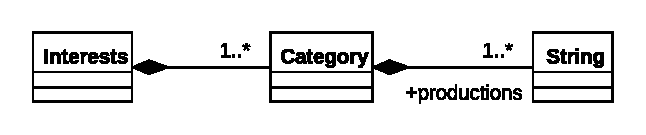
\includegraphics{images/paper/interests.eps}
 \caption{Interest Configuration Model}\label{fig:interest} 
 \end{center}
\end{figure}


As part of the experiment detailed in Section \ref{sec:exp_design} we need the ability to generate interest configurations for each grammar. We have developed a simple algorithm, depicted in \ref{alg:interest}, to do just that. The algorithm takes two parameters $G$ the initial grammar and $n$ the number of interest components to extract. Using this information, the algorithm constructs an empty list, $P$ which is then filled with the non-terminal symbols of the grammar. This list is then randomly shuffled and the top $n$ are selected and returned.

\begin{algorithm}[tb]
 \caption{Interest Configuration Generation}\label{alg:interest}

 \begin{algorithmic}[1]
   \Procedure{Generate}{$G$, $n$}
   \State $P \longleftarrow [\,]$
   \State $P \longleftarrow G.\Sigma / G.S$
   \State \Call{Shuffle}{$P$}
   \State \Return $P[1..n]$
   \EndProcedure
 \end{algorithmic}
\end{algorithm}

\section{Tolerization}

\begin{algorithm}
 \caption{Tolerization}
 \begin{algorithmic}[1]
  \Procedure{Tolerization}{$G,I$}
  
  \EndProcedure
 \end{algorithmic}

\end{algorithm}

\section{Bounding The Seas}

\begin{algorithm}
 \caption{BoundingTheSeas}
 \begin{algorithmic}[1]
  \Procedure{BoundingTheSeas}{$G,I$}
  
  \EndProcedure
 \end{algorithmic}

\end{algorithm}

\section{Bridgization}

\begin{algorithm}
 \caption{Bridgization}
 \begin{algorithmic}[1]
  \Procedure{Bridgization}{$G,I$}
  
  \EndProcedure
 \end{algorithmic}

\end{algorithm}

\chapter{Tool}

This chapter describes the design and implementation of the tool to automate the generation of Island, Tolerant, Bridge, and Bounded Seas grammars.

\section{Design}

\section{Implementation}

\chapter{Experimental Designs}

\section{Experiment 1: Evaluating Normalization}

\subsection{Goals, Hypotheses, Variables}

Following the GQM paradigm, research goal RG1 can be decomposed into the following set of research questions:

\begin{enumerate}[label={\textbf{RQ1.\arabic*}},left=.2in]
 \item What is the effect of each step in the normalization process on maintenance effort between the source grammar and the normalized grammar?
 
 \textbf{Rationale:}\textbf{}
 
 \item What is the effect of each step in the normalization process on the complexity between the source grammar and the normalized grammar?
 
 \textbf{Rationale:}\textbf{}
\end{enumerate}

In addition to these research questions we have selected the following metrics to assess the results of the approach used:

\begin{enumerate}[label={\textbf{M1.\arabic*}},left=.2in]
  \item Effort -- To assess the effort required to maintain a grammar, we utilize the Halstead Effort measure for grammars as defined by Power and Malloy \cite{power_metrics_2004}.
  \item Complexity -- To assess the complexity of a grammar, we utilize McCabe's Cyclomatic Complexity metric for grammars defined by Power and Malloy \cite{power_metrics_2004}.
\end{enumerate}

\subsection{Design}

\subsection{Experimental Units}

In these experiments, the experimental units are individual grammars selected from the Antlr4 \cite{parr_definitive_2012} grammar repository\footnote{\url{https://github.com/antlr/grammars-v4}}. The sys-verilog grammar was excluded because of errors while parsing it. At the time of this writing, the repository contained 198 individual grammars from a variety of general purpose and domain specific languages.

The process used to select the grammars for each experiment is depicted in Figure \ref{fig:selection_process} and works as follows. Initially, for each grammar in the repository we collected a combination of metadata and metric measurements. The metadata collected consists of the following information: the language represented by the grammar, the version of that language (if applicable) and the following metrics (selected from the metrics suite by Power and Malloy \cite{power_metrics_2004}):

\begin{itemize}
\item TERM -- the number of terminals.
\item VAR -- the number of defined non-terminals.
\item PROD -- the number of productions.
\item MCC -- McCabe's Cyclomatic Complexity.
\end{itemize}

Using the resulting measures, the grammar dataset was subdivided into three categories (Small, Medium, and Large) based on a statistical thresholding technique. This subdivision is based on the logarithm of PROD measures and yielded the following thresholds: Small-Medium: $10^{\mu_{PROD}-\sigma_{PROD}} = 10^{1.8404-0.5371} = 20.1084$ and Medium-High: $10^{\mu_{PROD}-\sigma_{PROD}} = 10^{1.8404+0.5371} = 238.4995$. Using these threshold each grammar is then grouped into one of the three categories. The size category then becomes a factor in the experimental model. 



\subsection{Data Collection Procedures}

Data collection is performed via the experiment execution system specifically developed for these studies. This system is controlled via the control files created during the experimental unit selection process. The data collection process follows the activity diagram depicted in Figure X, and operates as follows.

Initially, the control file is read into the system. Next, for each of the triples in this file, the following occurs: 1.) The normalizer process is setup for the experiment. 2.) The grammar to be normalized is located, read in, and parsed into an instance of the metamodel. 3.) The initial effort or complexity of the grammar is measured and recorded. 4.) The normalization process is applied, which results in a modified grammar. 5.) The effort or complexity of this normalized grammar is measured and recorded.

Once all experimental units have been processed, the results are exported to a data table. This process is repeated for each replication of each experiment. The results form each replication of each experiment are then combined into a single data table. The combined data table is then used during the analysis phase.

\subsection{Analysis Procedures}

\subsection{Validity Evaluation}

\section{Experiment 2: Evaluating Merging}

\subsection{Goals, Hypotheses, Variables}

This subsection describes the refinement of our initial research goal, defined in \ref{sec:introduction}, into a set of actionable research questions and metrics. Based on this set of research questions we also identified the variables used in statistical models driving our analytical procedures. We begin with the research questions and metrics.

Following the GQM paradigm, research goal RG2 can be decomposed into the following set of research questions:

\begin{enumerate}[label={\textbf{RQ2.\arabic*}},left=.2in]
 \item What is the effect that this process has on the maintenance effort between the source grammars and the grammar produced by this approach?

 \textbf{Rationale:} \textit{It is expected that the merging of grammar components will reduce the maintenance effort required.}

 \item What is the effect that this process has on the complexity between the source grammars and the grammar produced by this approach?

 \textbf{Rationale:} \textit{It is expected that the merging and reduction of grammar components will reduce the complexity of the grammar, thus making the grammar easier to understand and read.}
\end{enumerate}

\noindent In addition to these research questions we have selected the following metrics to assess the results of the approach used:

\begin{enumerate}[label={\textbf{M2.\arabic*}},left=.2in]
  \item Effort -- To assess the effort required to maintain a grammar, we utilize the Halstead Effort measure for grammars as defined by Power and Malloy \cite{power_metrics_2004}.
  \item Complexity -- To assess the complexity of a grammar, we utilize McCabe's Cyclomatic Complexity metric for grammars defined by Power and Malloy \cite{power_metrics_2004}.
\end{enumerate}

The dependent variables in the experiments, as indicated by the above research questions, are maintenance effort and complexity. Specifically, we are concerned with the change between the trivial merge state and the final grammar in terms of the effort and complexity of the grammar. Thus, the dependent variables of concern are:

\begin{itemize}
\item $\Delta HAL$ -- the change in Halstead Effort as measured after the normalization phase prior to the final merge phase, and after the final merge phase and before generating the output grammar.
\item $\Delta MCC$ -- the change in complexity as measured after the normalization phase prior to the final merge phase, and after the final merge phase and before generating the output grammar.
\end{itemize}

\noindent The independent variables we are concerned with are:

\begin{itemize}
\item Similarity Threshold -- the parameter guiding the similarity measurements used in the merging process. The values used in the experiments are 0.001, 0.25, 0.5, 0.75, and 1.0.
\item Size -- the size of the grammar as defined by measuring its number of productions (PROD) \cite{power_metrics_2004}, and threshold this value into three distinct categories: Small, Medium, and Large, as defined in Section \ref{sec:subjects}.
\end{itemize}

\subsection{Design}

To evaluate the approach we elected to conduct two experiments. The first experiment evaluates the effect the approach has on the maintenance effort necessary to maintain a merged grammar as compared to its combined source grammars. The second experiment evaluates the effect the approach has on the complexity of the merged grammar as compared to its combined source grammars. These experiments utilize a Factorial Design, with a single dependent variable ($\Delta HAL$, $\Delta MCC$), a treatment factor $Similarity Threshold$ and the grouping factor $Size$.

\subsection{Experimental Units}

\begin{table*}[tb]
\centering
\caption{Grammars randomly selected from each size category used in the experiments.}
\label{tbl:grammar_metrics}
\begin{tabular}{|c|l|}
\hline
Category & Grammars\tabularnewline
\hline
\hline
\multirow{2}{*}{S} & brainfuck, cmake, csv, inf, lcc, pdn,\tabularnewline
\cline{2-2}
 & properties, quakemap, sexpression, tsv, url, useragent\tabularnewline
\hline
\multirow{2}{*}{M} & cto, dart2, flatbuffers, fusion-tables, lua, pascal\tabularnewline
\cline{2-2}
 & python2, romannumerals, sgf, stacktrace, webidl, z-ops\tabularnewline
\hline
\multirow{2}{*}{L} & cql3, edif300, fortran77, idl, informix, java9\tabularnewline
\cline{2-2}
 & kotlin, objc-two-step, powerbuilder, rexx, sharc, swift2\tabularnewline
\hline
\end{tabular}
\end{table*}

This section describes the experimental units and the process used to select them. In these experiments, the experimental units are pairs of grammars selected from the Antlr4 \cite{parr_definitive_2012} grammar repository\footnote{\url{https://github.com/antlr/grammars-v4}}. The sys-verilog grammar was excluded because of errors while parsing it. At the time of this writing, the repository contained 198 individual grammars from a variety of general purpose and domain specific languages.

The process used to select the grammar pairs for each experiment is depicted in \ref{fig:selection_process} and works as follows. Initially, for each of the grammars in the repository we collected a combination of metadata and metric measurements. The metadata collected consists of the language represented by the grammar, the version of that language (if applicable) and the following metrics (selected from the metrics suite by Power and Malloy \cite{power_metrics_2004}):

\begin{itemize}
\item TERM -- the number of terminals.
\item VAR -- the number of defined non-terminals.
\item PROD -- the number of productions.
\item MCC -- McCabe's Cyclomatic Complexity.
\end{itemize}

\begin{figure}[tb]
 \centering
 \subfloat[Experimental unit selection process.]{
  \label{fig:selection_process}
  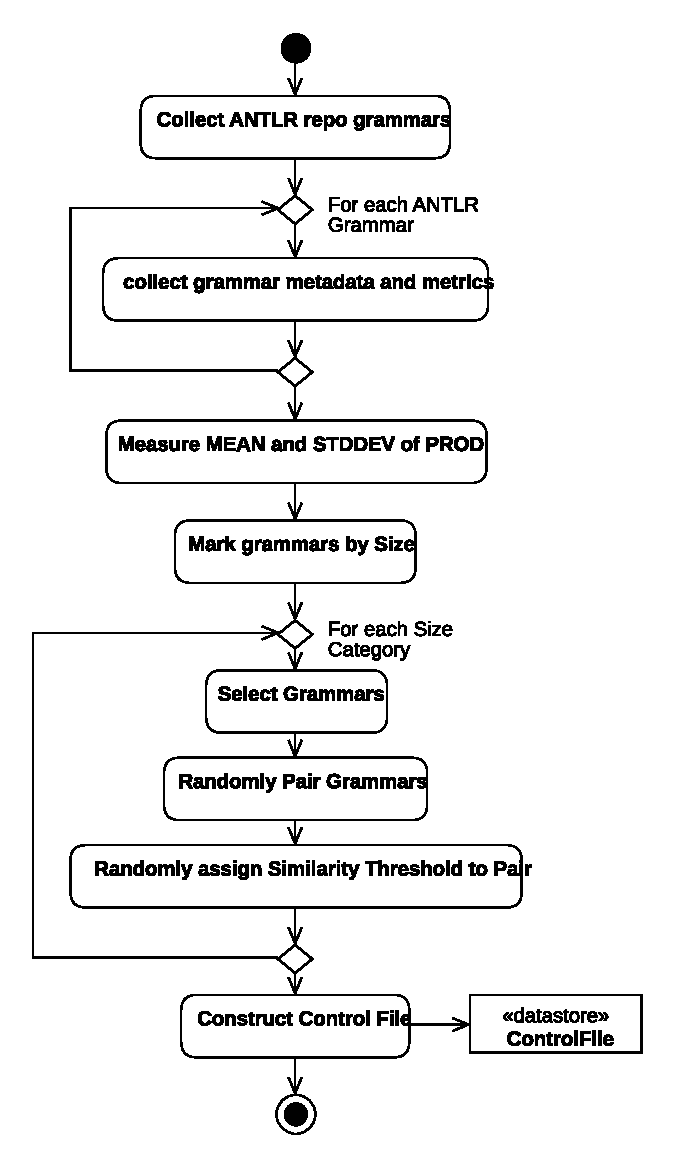
\includegraphics[width=.49\textwidth]{images/paper/selection_process.eps}
 }
 \subfloat[Data collection procedure.]{
  \label{fig:dc_proc}
  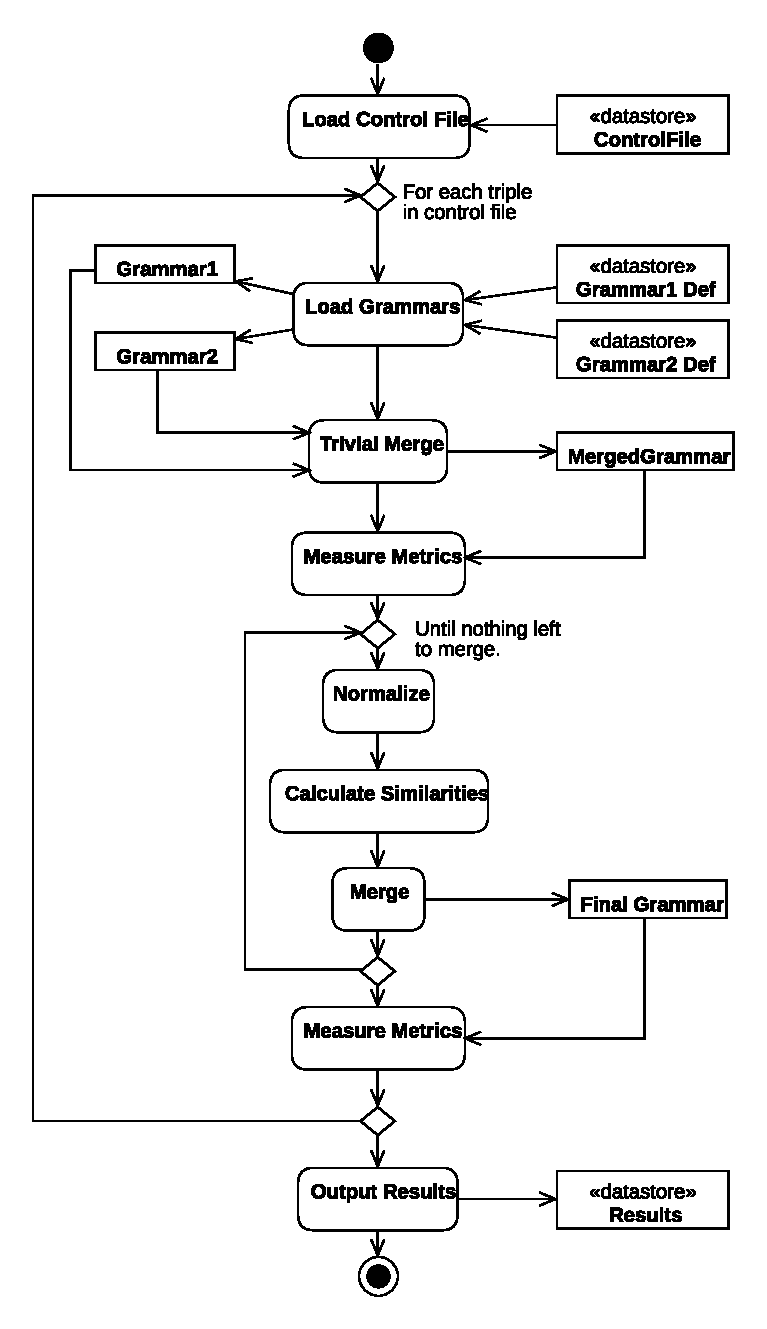
\includegraphics[width=.49\textwidth]{images/paper/data_collect.eps}
 }
 \caption{Activity diagrams for the (a) experimental unit selection process and (b) the data collection process.}
\end{figure}

Using the resulting measures of these metrics, the grammar dataset was subdivided into three categories (Small, Medium and Large) based on the logarithm of PROD (as the values were log-normal distributed). This subdivision was based on statistically construction thresholds, as per Lanza and Marinescu \cite{lanza_object-oriented_2011}. Category threshold values are defined as: Small-Medium: \(10^{\mu_{PROD} - \sigma_{PROD}} = 10^{1.8404 - 0.5371} = 20.1084\) and Medium-High: \(10^{\mu_{PROD} + \sigma_{PROD}} = 10^{1.8404 + 0.5371} = 238.4995\). Using these thresholds each grammar is then grouped into one of the three categories.

Using these categories as the grouping factor in the experiments, we can then begin the sampling process. As we have selected a $3\times 5$ factorial design, each replication of each experiment requires 15 grammar pairs (5 per size category). Based on our replication analysis (described in Section \ref{sec:analysis_proc}) we have identified a need for a total of 5 replications. Thus, For each size category we require a total of 50 grammar pairs per experiment yielding a need for 100 total grammar pairs. To meet this requirement we randomly select (without replication) 12 grammars, per size category. From these 12 grammars there are $12 \choose 2$ = 66 combinations (without replication) of which we randomly select 5 pairs per replication per experiment. The grammars selected and their pairings per experiment/replication are depicted in Table \ref{tbl:grammar_metrics}.

Once the grammar pairs are selected, they are assigned a treatment value for use during the experiment execution and data collection phase. For each size category in each replication of each experiment, the set of five grammar-pairs are assigned, at random, a level of the similarity threshold treatment. The possible levels that can be assigned are 0.001, 0.25, 0.5, 0.75, and 1.0 (where 1.0 is the control level).

Finally, the data generated as part of the selection process is used to construct an experiment control file. This file is used to direct the experimental execution system and to ensure the validity of the process. Each control file is simply an ordered set of triples. Where, each triple consists of the following information:

\begin{itemize}
\item Grammar Pair - the pair of grammars to be merged together, as selected during the selection phase.
\item Treatment - the similarity threshold value assigned to the grammar pair during the selection phase.
\item Size - value of the size category, for use in constructing the data table.
\end{itemize}

\noindent Each replication of each experiment has a separate control file to control its execution. Thus, for each replication of each experiment, the control file triples are created and put into a list which is then randomized. This randomized list is then output to a file which is later read in by the experimental execution system.

\subsection{Data Collection Procedures}

Data collection is performed via the experiment execution system specifically developed for this study. This system is controlled via the control files created during the experimental unit selection process. The data collection process follows the activity diagram depicted in Figure \ref{fig:dc_proc}, as follows.

Initially, the control file is read into the system. Then, for each of the triples in the list, the following occurs: 1.) The selected similarity threshold value is applied. 2.) The grammars located, read in, and trivially merged together. 3.) The combined grammar's effort or complexity is then measured and recorded. 4.) The final merging process is applied resulting in the final grammar. 5.) The resulting grammar's effort or complexity is then measured and recorded.

Once all experimental units have been processed the results are exported to a data table. This process is repeated for each replication of each experiment. The results from each replication of each experiment are then combined into a single data table. The combined data table is then used during the analysis phase.

\subsection{Analysis Procedures}

As described in Section \ref{sec:experimental_design}, both experiments utilize a Factorial design \cite{montgomery_design_2013}. Typically, a factorial design experiment will utilize ANOVA to determine if there is a difference between the effects of the factors. In this case, the statistical model used is as follows:

\[y_{ijk} = \mu + st_i + size_j + (st * size)_{ij} \epsilon_{ijk}\]

\noindent Where:
\begin{itemize}
\item $y_{ijk}$ is the kth value of the observation (either $\Delta MCC$ or $\Delta HAL$) associated with the ith similarity threshold level and jth size level.
\item $\mu$ is the baseline mean
\item $st_{i}$ is the ith level of similarity threshold effect.
\item $size_{j}$ is the jth level of size effect.
\item $(st * size)\_{ij}$ is the similarity threshold * size interaction effect.
\item $\epsilon_{ijk}$ is the random error of the kth observation from the (i, j)th cell.
\end{itemize}

\noindent The hypotheses to be tested in this case are as follows:

\begin{itemize}
\item $H_{1,0}$ : The effect of the levels of the interaction term are equal.
\item $H_{1,A}$ : There is at least one difference between interaction level effects.
\item $H_{2,0}$ : The effects of the levels of similarity threshold are equal.
\item $H_{2,A}$ : There is at least one difference between similarity threshold level effects.
\item $H_{3,0}$ : The effects of the levels of size are equal.
\item $H_{3,A}$ : There is at least one difference between size level effects.
\end{itemize}

ANOVA has several assumptions that must first be verified. First, is the assumption of homogeneity of variance. To evaluate this assumption, we will use Levene's Test \cite{levene_robust_1960}. The next assumption is that both the factors and errors are normally distributed. To verify this assumption, we will use the Anderson-Darling Test for Goodness of Fit \cite{anderson_test_1954} to the normal distribution for both the errors and factor effects. Finally, there is the assumption of independence of the observations, which is valid due to the nature of the process.

In the case of any violations of these assumptions we will attempt to correct the violation. In the case that the assumptions are violated beyond the capability to correct, we will be forced to utilize a non-parametric approach. Specifically, we will use a permutation F-test \cite{higgins_introduction_2004}, in place of ANOVA. The permutation F-test also has a set of assumptions that must be met prior to use. ... The model for the permutation F-test is the same as that of ANOVA.

In either case, the next step is to conduct the hypothesis test and make a decision. In this case we have selected an $\alpha$ threshold of 0.95. In the case that we reject $H_{1,0}$ we will then conduct a multiple-comparison procedure to compare the individual effects of each level of the similarity threshold factor. In these experiments the similarity threshold level of 1.0 to be the control (as noted in Section \ref{sec:design}). We have selected to pair Dunnett's \cite{dunnett_multiple_1955} multiple comparison procedure if ANOVA is used, and Steel's \cite{steel_multiple_1959} multiple comparison procedure (a non-parametric technique analogous to Dunnett's) if using the permutation F-test. Both of these comparison procedures control the error for multiple comparisons and allow the ability to compare against a control. In the case of Dunnett's Test we will be evaluating the following hypotheses:

\begin{itemize}
\item $H_{4,0}$ : There is no difference between the mean effects of similarity threshold effects and control effect.
\item $H_{4,A}$ : There is a difference between at least one similarity threshold level and control.
\end{itemize}

\noindent In the case of Steel's Test we will be evaluating the following hypotheses:

\begin{itemize}
\item $H_{4,0}$ : There is no difference between the median effects of similarity threshold effects and control effect.
\item $H_{4,A}$ : There is a difference between at least one similarity threshold level and control.
\end{itemize}

\noindent For either of these tests we will use an $\alpha$ threshold of 0.95.

Additionally, we are interested if there is a strict order of the effect on $\Delta HAL$ or $\Delta MCC$ for the levels of the similarity threshold factor. To evaluate this we have selected to utilize the Jonhckheer's trend test. This is a non-parametric test to determine if there is an \textit{a priori} ordering within independent samples \cite{jonckheere_distribution-free_1954}. The hypotheses to be tested are as follows:

\begin{itemize}
\item $H_{5,0}$ : There is no difference in median effects of the similarity threshold levels.
\item $H_{5,A}$ : There is a increasing trend in the effects of the similarity threshold levels, with at least one being a strict inequality.
\end{itemize}

Finally, we will also conduct a sample size analysis to determine the number of repetitions necessary to achieve the power level necessary for the experiments.

\subsection{Validity Evaluation}

This subsection details the procedures put in place as part of the experimental design to ensure the validity of the results. As per Wohlin et al. \cite{wohlin_experimentation_2012} we are concerned with conclusion, internal, construct, and external validity.

\subsubsection{Conclusion Validity}

The following characteristics of our experiments and data help to ensure the conclusion validity of this study. First due to the nature of the data we have put into place techniques which validate the assumptions of our statistical tests, and in the case of that we are unable to correct violations of these assumptions we have selected alternative analysis procedures. As part of this study several metrics are used to evaluate the selected grammars and those generated by our proposed technique. To ensure that the accuracy of the implementation of these metrics, they have been thoroughly tested prior to use. To ensure the accurate operation of the experiments we have implemented and tested an experimental execution system. For each experiment we are utilizing multiple comparison procedures, both of which have been selected such that they utilize proper error correcting procedures. Finally, due to the nature of the experiments there are no issues in the experimental setting that will cause random irrelevancies.

\subsubsection{Internal Validity}

The following characteristics of our experiments and data help to ensure the internal validity of this study. First, due to the nature of the experimental units and experimental system the timing of experiment execution has no effect on the outcome. Second, due to the nature of the experimental units there are no social concerns affecting the internal validity. Third, the experimental unites are grammars generated by the combination of existing grammars a process which does not affect the source grammars and which leaves no lasting effect to influence the outcome when repeating the same experiment. Fourth, We have selected grammars that are representative for population of ANTLR grammars and for different sizes, but which may be under-representative of grammars in general. Fifth, the selection, assignment and analysis procedures used in these experiments have been designed to ensure that there is no ambiguity regarding the direction of causal influence.

\subsubsection{Construct Validity}

The following characteristics of our experiments and data help to ensure the construct validity of this study. First, the nature of the experimental units preclude social issues affecting construct validity. Second, the design of the experiments and the technique being evaluated prevents both mono-operation and mono-method biases. Third, there are no issues due to inadequate preoperational explication or confounding constructs. Fourth, the use of size categories for source grammars is designed to evaluate the spectrum of grammars rather than simply testing whether the technique works on grammars. Fifth, the design of the experiments and the experiment execution system prevents interaction of treatments. Sixth, due to the nature of the technique and the experimental process the source grammars are left unaffected.

\subsubsection{External Validity}

The following characteristics of our experiments and data help to ensure the external validity of this study. The selection of simple languages (such as the group of small languages) not currently in use in industry would pose a threat to external validity, but this is offset by the inclusion of the other languages from both the medium and large groups. Second, we restrict our internal representations to BNF, but we do include the ability to utilize ANTLR grammars which are currently used in practice. Yet, because we do not include grammars in other formalisms (i.e., SDF \cite{heering_syntax_1989} and TXL \cite{cordy_txl_2004}) used in practice a threat to external validity still remains. Finally, the nature of the experiment precludes an effect due to the date or time of the application of the treatment.

\section{Experiment 3: Evaluating Islandization}

This section describes the study design for the experiment used to evaluate the multilingual island grammar generation approach from @sec:approach. In developing this study we followed the guidance of Runeson [@http://zotero.org/users/1776655/items/IIF2B7Z7] and Yin [@http://zotero.org/users/1776655/items/KQJDZFIR]. The following subsections detail the research questions, case selection criteria, data collection procedures, and analysis procedures used.

\subsection{Goals, Hypotheses, Variables}

In the spirit of the GQM, we have further refined this goal into a series of directly answerable questions and their underlying rationale. The questions are as follows:

\begin{enumerate}[left=1em,label=\bfseries RQ\arabic*:]
  \item How can we automate the combination of languages into a single island grammar?\\
  \textbf{Rationale:}
  \item What is the comparative readability of merged grammars?\\
  \textbf{Rationale:}
  \item What is the comparative usability of merged grammars?\\
  \textbf{Rationale:}
  \item What is the comparative maintainability of merged grammars?\\
  \textbf{Rationale:}
\end{enumerate}

To facilitate answering these questions we have also defined a series of metrics, as follows:

\begin{enumerate}[left=1em,label=\bfseries M\arabic*:]
  \item McCabe Cyclomatic Complexity (MCC) a measure of the complexity of a grammar $\mathcal{G}$. \\
  \textbf{Rationale:} A higher complexity represents difficulty in comprehension of the grammar and difficulty in maintaining the grammar. An island grammar is expected to have a lower complexity value than their input grammars.
  \item Halstead Effort (HAL) a measure of effort necessary to maintain grammar $\mathcal{G}$. \\
  \textbf{Rationale:} Similar to MCC, but provides a means by which the MCC is effectively relativised. Island grammars are expected to have a lower complexity and thus lower HAL than their input grammars.
  \item Size of the Set of Input Grammars (Size(G)) the cardinality of the grammars used as input for the island grammar generation. \\
  \textbf{Rationale:} The size of the input grammar set is a key factor in the overall complexity of the generated island grammar and thus should be accounted for.
  \item Size of the Set of Interest Components per grammar (Size(I)) the cardinality of the interest component set used for each grammar acting as input to the island grammar generation algorithms. \\
  \textbf{Rationale:} The size of the interest component set for each grammar used as input for an island grammar is a key factor in the overall complexity of the generated island grammar and thus should be accounted for.
  \item $version(\mathcal{G})$ indicative of the version of the language the grammar $\mathcal{G}$ recognizes. This is a qualitative measure with text data.\\
  \textbf{Rationale:}
\end{enumerate}

The following describes the data to be collected, the data collection process, and how this data is to be stored.
First, we describe the data that must be collected. For each grammar under study, we extract the Grammar name, language version,
Grammar type, readability score, usability score, and maintainability score for each grammar measured from the Grammar Measure Database, as collected by the tool presented in Section \ref{sec:approach}. The data is then accumulated into a table, similar to the example shown in Table \ref{tbl:example}, with the following specifications:

\begin{itemize}
\item Each row of the represents data associated with a specific grammar set.
\item The first column is the grammar set identifier.
\item The second column represents the method for island grammar generation.
\item The third column represents size of the grammar set.
\item The fourth column represents the size of the interest set of each grammar in the set.
\item The fifth column represents the calculated complexity of the generated island grammar.
\item The sixth column represents the average complexity of the grammar set.
\item The seventh column represents the calculated effort of the generated island grammar.
\item The eighth column represents the average effort of the grammar set.
\end{itemize}

The data that is collected then breaks down into the following \textit{independent} and \textit{dependent} variable sets. The independent variables representing the properties of concern for the grammar sets are: Technique, Size(G), and Size(I). The levels associated with technique are \textit{Naive} and \textit{MIGG} depending on the assignment of the set to either the Naive or MIGG approaches for island grammar generation. The levels associated with Size(G) are 2, 5, or 10 which represent a sample of the possible number of grammars to be combined. Finally, the levels associated with Size(I) are 2, 5, and 10 which represent a sample of the possible number of interest components that could be selected from a particular grammar. The dependent variables of concern are $\Delta MCC$ and $\Delta HAL$. $\Delta MCC$ is the difference between the MCC of the generated grammar and the Average MCC of the source grammars. $\Delta HAL$ is the difference between the HAL of the generated grammar and the Average HAL of the source grammars.

\begin{table*}[tb]
\centering
\caption{Example data table for this study.}\label{tbl:example}
\begin{tabular}{|c|c|c|c|c|c|c|c|}
\hline
Grammar Set & Method & Size(G) & Size(1) & $MCC_{IG}$ & $MCC_{avg}$ & $HAL_{IG}$ & $HAL_{avg}$\\
\hline
\hline
1 & Naive & 2 & 2 & 0.95 & 0.95 & 0.95 & 0.75\\
\hline
1 & MIGG & 2 & 5 & 0.75 & 0.95 & 0.95 & 0.925\\
\hline
\end{tabular}
\end{table*}

Based on the research questions posed above and the variables utilized to evaluate the grammars, we have constructed the following sets of hypotheses. The first set is based on evaluating the change in complexity of the grammars when reduced to a combined Island Grammar. \textit{We expect that when a selection of languages are combined into an Island Grammar with a set of interests imposed, the generated language should be less complex than the average complexity of languages in the input set.} The statistical hypotheses used to test are:

\begin{enumerate}[left=1em,label=H\textsubscript{\arabic*,0} :]
 \item An increase in the number of grammars shows a decrease in average $\Delta MCC$
 \item An increase in the number of interests shows a decrease in average $\Delta MCC$
 \item There is a difference in average $\Delta MCC$ between the techniques used to generate island grammars, when controlling for $Size(G)$ and $Size(I)$
\end{enumerate}

The second set is based on evaluating the change in effort to maintain the grammars when reduced to a combined Island Grammar. \textit{We expect that when a selection of languages are combined into an Island Grammar with a set of interests imposed, the generated language should less effort to maintain than the average effort of languages in the input set.} The statistical hypotheses used to test this are:

\begin{enumerate}[left=1em,label=H\textsubscript{\arabic*,0} :,start=4]
 \item An increase in the number of grammars shows a decrease in the average $\Delta HAL$
 \item An increase in the number of interests shows a decrease in the average $\Delta HAL$
 \item There is a difference in average $\Delta HAL$ between the techniques used to generate island grammars, when controlling for $Size(G)$ and $Size(I)$
\end{enumerate}

\subsection{Design}

To gain the most from this experiment, we have elected to use a factorial design. Thus, since we have 2 factors with 3 levels and 1 factor with 2 levels, each replication will need 36 sets of grammars. Furthermore, because the Size(G) variable is based on the number of grammars that are included in the set, we thus need 12 sets at each level of Size(G). Due to this, we need 204 grammars per replication. To gain the most from this experiment we will conduct 3 replications of the experiment, meaning that we require 612 individual grammars.

\subsection{Experimental Units}

This section describes the methods of subject sampling and group allocation. For the purposes
of this experiment the experimental subjects are grammars representing software languages. Furthermore,
as we are concerned with evaluating MIGG from the perspective of creating static and dynamic analysis tools,
we have imposed the following restrictions on the types of grammars we are interested in:

\begin{itemize}
\item A Grammar may be considered a viable case, if it contains a minimum of 15 different productions.

  \textbf{Rationale}: the grammar should be more than a simple toy grammar.

\item A Grammar may be considered a viable case, if it defines a known and oft used programming language.

  \textbf{Rationale}:
\end{itemize}

With these restrictions in mind we decided to utilize the Grammar Zoo  collection as initial pool from which to select our grammars. Grammar Zoo (at the time of this writing) contains 1029 entries consisting of grammars for a variety of programming languages. With the exception of a few languages most in the collection represent languages currently used in practice by Software Engineers (e.g., Java, Python, Haskell, Dart, etc.).

As noted in Section \ref{sec:design} we will need 612 individual grammars to conduct this experiment. These grammars are selected as follows: Initially, 604 grammars are randomly selected from the initial 1029 grammars in Grammar Zoo using a simple random sampling approach. This set is then randomly partitioned into 3 subsets of 104 grammars representing each of the individual replications of the experiment. Within each replication, the grammars are randomly assigned to treatment groups based on the Size(G) characteristic. For each of the treatment groups, a Size(I) level is assigned. Based on this value, a new Interest Configuration for each of the languages is generated using the Interest Configuration generation algorithm presented in Section \ref{sec:approach}. Finally, each treatment group is randomly assigned a generation approach for use in the evaluation process.

\subsection{Instrumentation}

As part of the experimental design measures for metrics M1--M5 must be collected for each generated island grammar. To do this, the tool described in Section \ref{sec:tool_design} provides this capability via implementations of the GrammarMetric depicted in Figure \ref{fig:model}. During program operation, these measures are stored in a database and are retrieve and added to a data table for processing in the analysis phase of the experiment.

\subsection{Data Collection Procedures}

\begin{figure}[tb]
\centering
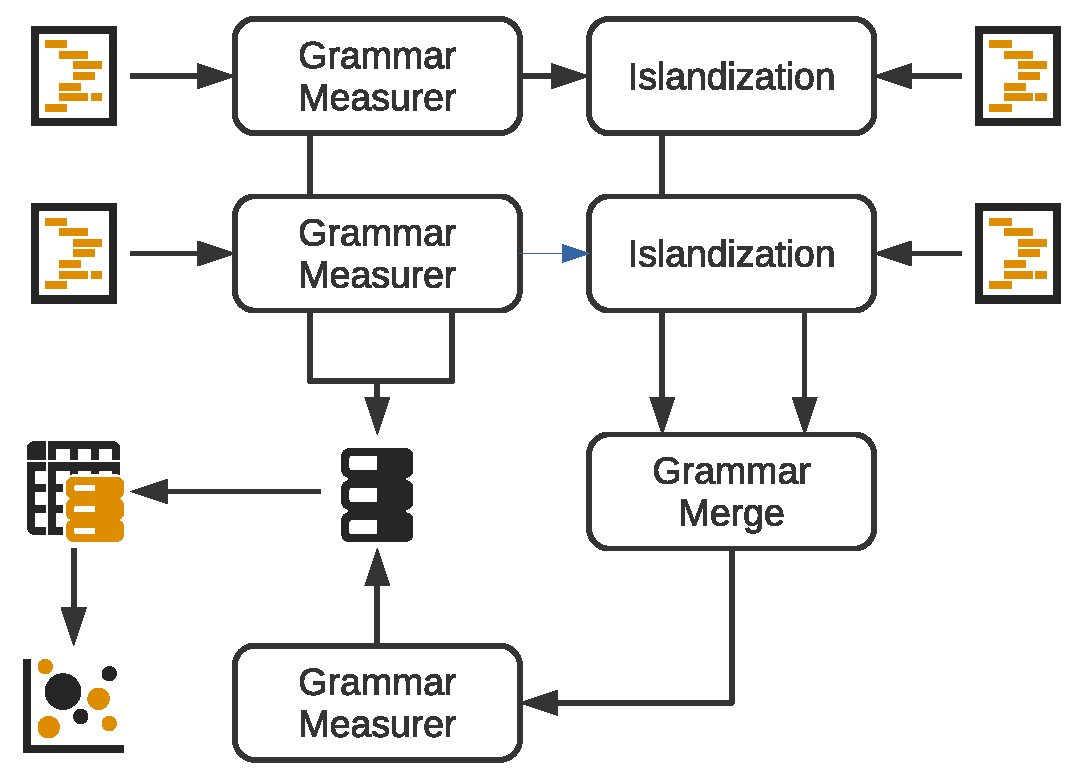
\includegraphics[width=\textwidth]{images/paper/dc_pair.eps}
\caption{Data collection process for evaluating multilingual grammar islandization process.}\label{fig:dc_pair}
\end{figure}

In this study, evaluating the effects of islandization and merging process to develop multilingual island grammars we use the process depicted in Figure \ref{fig:dc_pair}. This process follows the path identified in Figure \ref{fig:dc_pair} by the numbers encircled in orange, as follows:

\begin{enumerate}
\item Initially each grammar is loaded by the Grammar Loader and its data is extracted into the meta model depicted in Figure \ref{fig:model}.
\item A lattice of all combinations of grammars is generated to evaluate the groupings of languages into island grammars.
\item The quality metrics from the quality model are measured on the grammar, and
\item stored in the database.
\item The grammar is then transformed using the \textit{islandization}.
\item This requires that the interest configuration for that grammar be loaded.
\item The generated island grammar is then measured using the same metrics from step 2.
\item For the current combination approach, the set of grammars are then merged to generate a multilingual island grammar.
\item This grammar is then measured, using the same approach as in step 2, and the data is stored to the database.
\item For each grouping defined in the current partitioning of grammars, the IQR of the individual island grammars is measured, and stored to the database.
\item For the partitioning the average IQR is then calculated and stored to the database. This process restarts at step 1, until there are no partitions left.
\item Once all partitions have been processed, the data for all partitions is extracted into a data table ready for analysis.
\end{enumerate}

\subsection{Analysis Procedures}

The following analysis procedures are used in answering the questions posed in Section \ref{sec:goals}. In the first part of this study we have naturally paired samples of data. Given this, we are able to utilize very rudimentary analyses to answer the questions.

For questions RQ3 -- RQ5

\noindent The results will be in the form of confidence intervals defined at the $\alpha = 97.5\%$ confidence level.

\subsubsection{Exploratory Data Analysis}

To understand the data collected during experimental operation we used a number of basic statistical analyses. Specifically, to understand the dispersion and typical values of the dependent variables we evaluated the mean and standard deviations of $\Delta MCC$ and $\Delta HAL$. Furthermore, to understand the nature of the relationships between the dependent and independent variables we evaluated the correlations between all variables in the experiment. Furthermore, we can graphically display all of this information in a lattice structure.

\subsubsection{Primary Analyses}

The primary analyses used in the experiment are designed to evaluate the hypotheses identified in \ref{sec:goals}. The experimental design is a factorial design and thus would be typically evaluated using an ANOVA model. But, ANOVA has several assumptions which if not met leads to a higher chance of Type-II error. To evaluate these assumptions we will be utilizing the following tests:

\begin{itemize}
\item To evaluate the normality of the data we will use the Shapiro-Wilk test [@http://zotero.org/users/1776655/items/XDSBUJ53] for normality.
\item To evaluate the homogeneity of variance we will use Levene's test for homogeneity of variance [@http://zotero.org/users/1776655/items/QUGJ536S].
\item Given the experimental approach we know that the samples are drawn independently and sampled randomly.
\end{itemize}

In the event that the assumption of the homogeneity of variance is violated but the data is normally distributed, we will apply a weighted variance approach to correct the model. On the other hand, if both assumptions are violated, we will simply return to utilizing the nonparametric Wilcoxson Rank-Sum [X] variant of the test. For both experiments evaluating HAL and MCC we will use the following model.
\[ y_{ijkl} = \mu + \tau_{ijk} + \epsilon_{ijkl} \]

\noindent Where, $y_{ijkl}$ is the observed value of HAL or MCC for the given treatment combination of {ijk} and error {l}. $\mu$ is the base line mean value of the MCC or HAL. $\tau_{ijk}$ is the treatment value for the $i^{th}$ level of $Method$, the $j^{th}$ level of $Size(G)$ and $k^{th}$ level of $Size(I)$. Finally, $\epsilon_{ijkl}$ is the error term representing random error to be controlled for. In the case of both of these experiments we are concerned with determining whether there is any difference due to different treatments, which leads to the following statistical tests:

\begin{enumerate}[left=1em,label=H\textsubscript{\arabic*,0} :]
 \item There is no difference in mean $\Delta MCC$
 \item There is no difference in mean $\Delta HAL$
\end{enumerate}

\begin{enumerate}[left=1em,label=H\textsubscript{\arabic*,A} :]
 \item There is at least one difference in $\Delta MCC$
 \item There is at least one difference in $\Delta HAL$
\end{enumerate}

\noindent In both cases ANOVA and the Rank-Sum based approach simple detect if there is a difference in the means, but does not inform us as to which variable lead to this difference. Thus, in order to detect the difference we will be applying the Tukey-HSV [@http://zotero.org/users/1776655/items/64U6XBSU] analysis to find difference in all means. Additionally, to better understand the effects of individual variables on $\Delta MCC$ and $\Delta HAL$ we will use the following ...

\subsection{Validity Evaluation}

\subsubsection*{Conclusion Validity}

\subsubsection*{Internal Validity}

\subsubsection*{Construct Validity}

\subsubsection*{External Validity}

\section{Experiment 4: Evaluating Tolerization}

\subsection{Goals, Hypotheses, Variables}

\subsection{Design}

\subsection{Experimental Units}

\subsection{Data Collection Procedures}

\subsection{Analysis Procedures}

\subsection{Validity Evaluation}

\section{Experiment 5: Evaluating Bounding the Seas}

\subsection{Goals, Hypotheses, Variables}

\subsection{Design}

\subsection{Experimental Units}

\subsection{Data Collection Procedures}

\subsection{Analysis Procedures}

\subsection{Validity Evaluation}

\section{Experiment 6: Evaluating Bridgization}

\subsection{Goals, Hypotheses, Variables}

\subsection{Design}

\subsection{Experimental Units}

\subsection{Data Collection Procedures}

\subsection{Analysis Procedures}

\subsection{Validity Evaluation}

\chapter{Results}

\section{Experiment 1: Evaluating Normalization}

\subsection{Descriptive Statistics}

\subsection{Hypothesis Testing}

\section{Experiment 2: Evaluating Merging}

\subsection{Descriptive Statistics}

This subsection describes the data collected via a series of descriptive statistics. Table \ref{tbl:descriptive} shows the mean values of $\Delta HAL$ and $\Delta MCC$ for each value of the size category in the respective experiments. Along with this table the dispersion of the both $\Delta HAL$ and $\Delta MCC$ across size and similarity threshold values is displayed in Figure \ref{fig:hal_box} and \ref{fig:mcc_box}, respectively.

\begin{table}[tb]
\centering
\caption{Descriptive Statistics.}
\label{tbl:descriptive}
\begin{tabular}{lrr}
\hline
\textbf{Size Category} & \textbf{Mean $\Delta HAL$} & \textbf{Mean $\Delta MCC$}\tabularnewline
\hline
Small & 1290.2 & 32.32\tabularnewline
Medium & 18573 & 112.7\tabularnewline
Large & 149854 & 842.4\tabularnewline
\hline
\end{tabular}
\end{table}

\begin{figure}[tb]
 \centering
 \subfloat[$\Delta Hal$ experiment Q-Q plots.]{
   \label{fig:ex1_qqplots}
   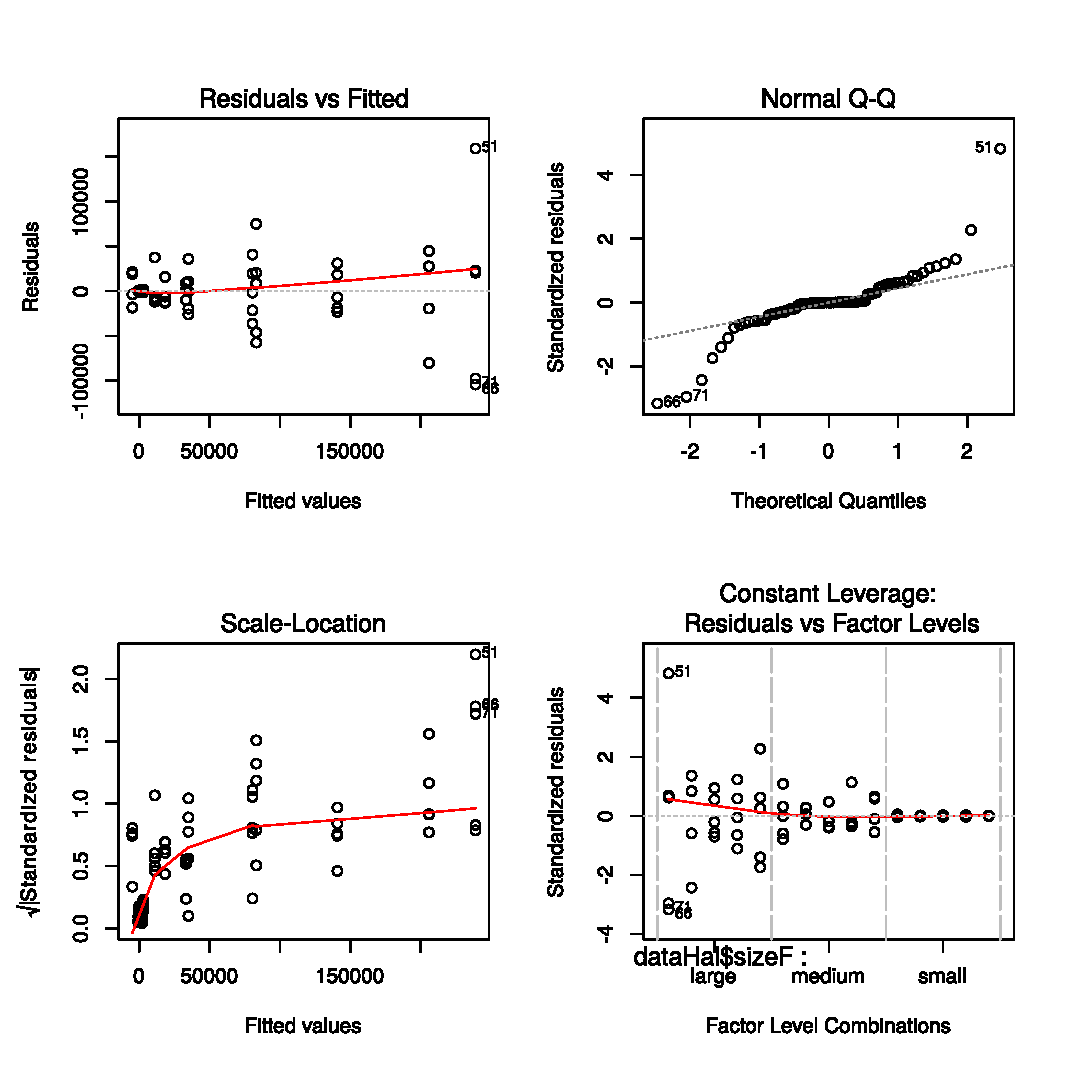
\includegraphics[width=.49\textwidth]{images/paper/results/ex1_qqplots.eps}
 }
 \subfloat[$\Delta MCC$ Experiment Q-Q plots.]{
   \label{fig:ex2_qqplots}
   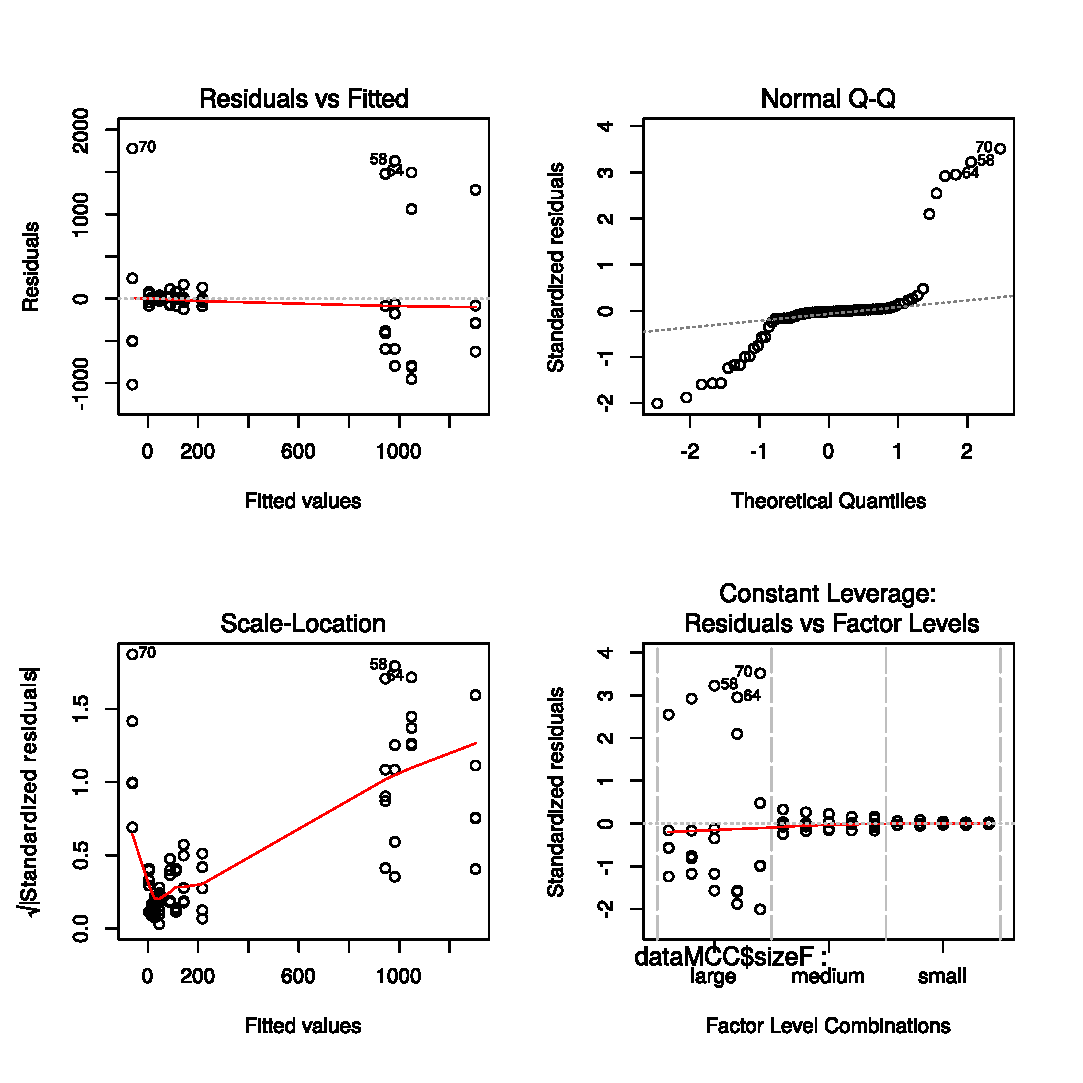
\includegraphics[width=.49\textwidth]{images/paper/results/ex2_qqplots.eps}
 }
 \qquad
 \subfloat[$\Delta HAL$ Boxplots.]{
   \label{fig:hal_box}
   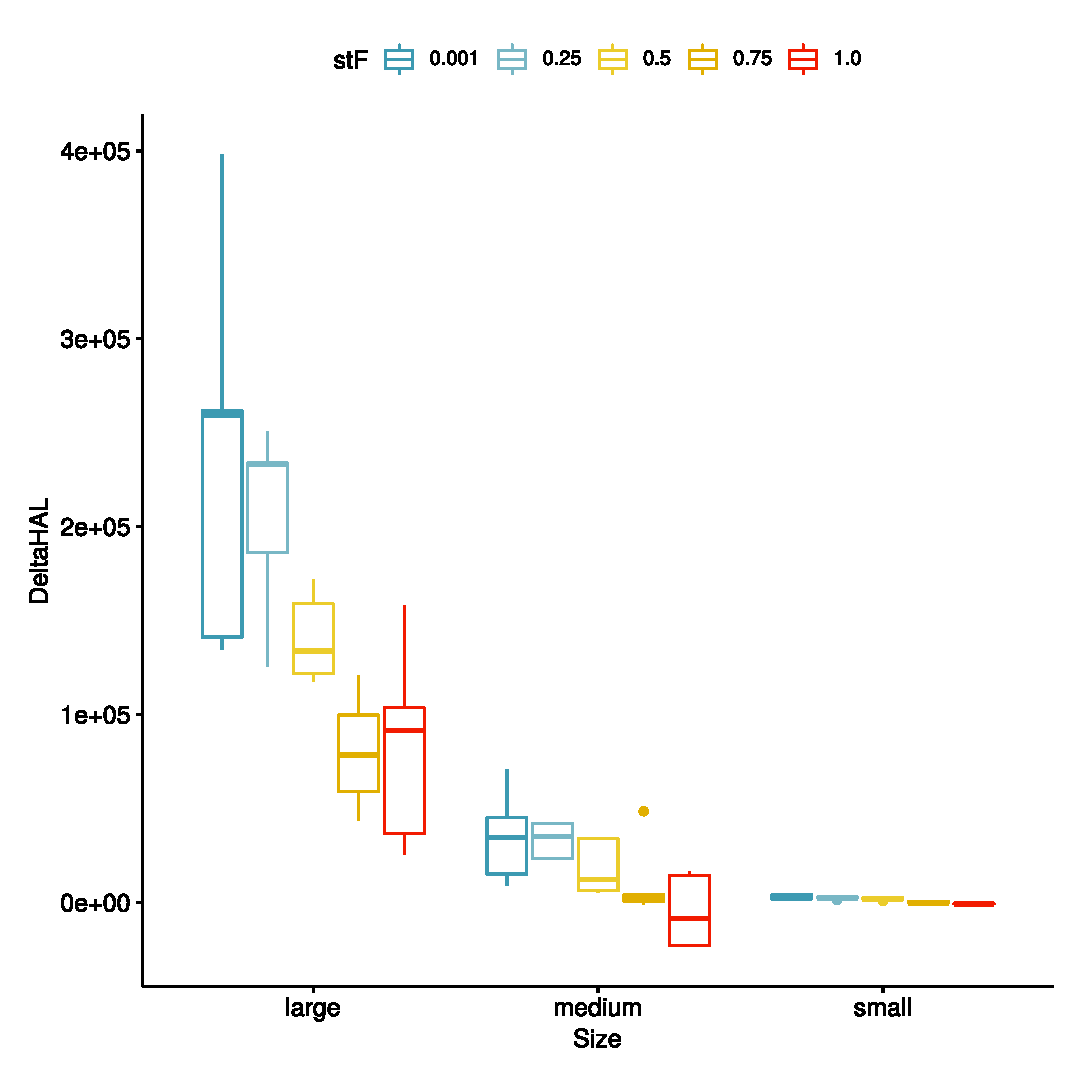
\includegraphics[width=.49\textwidth]{images/paper/results/hal_box.eps}
 }
 \subfloat[$\Delta MCC$ boxplots.]{
   \label{fig:mcc_box}
   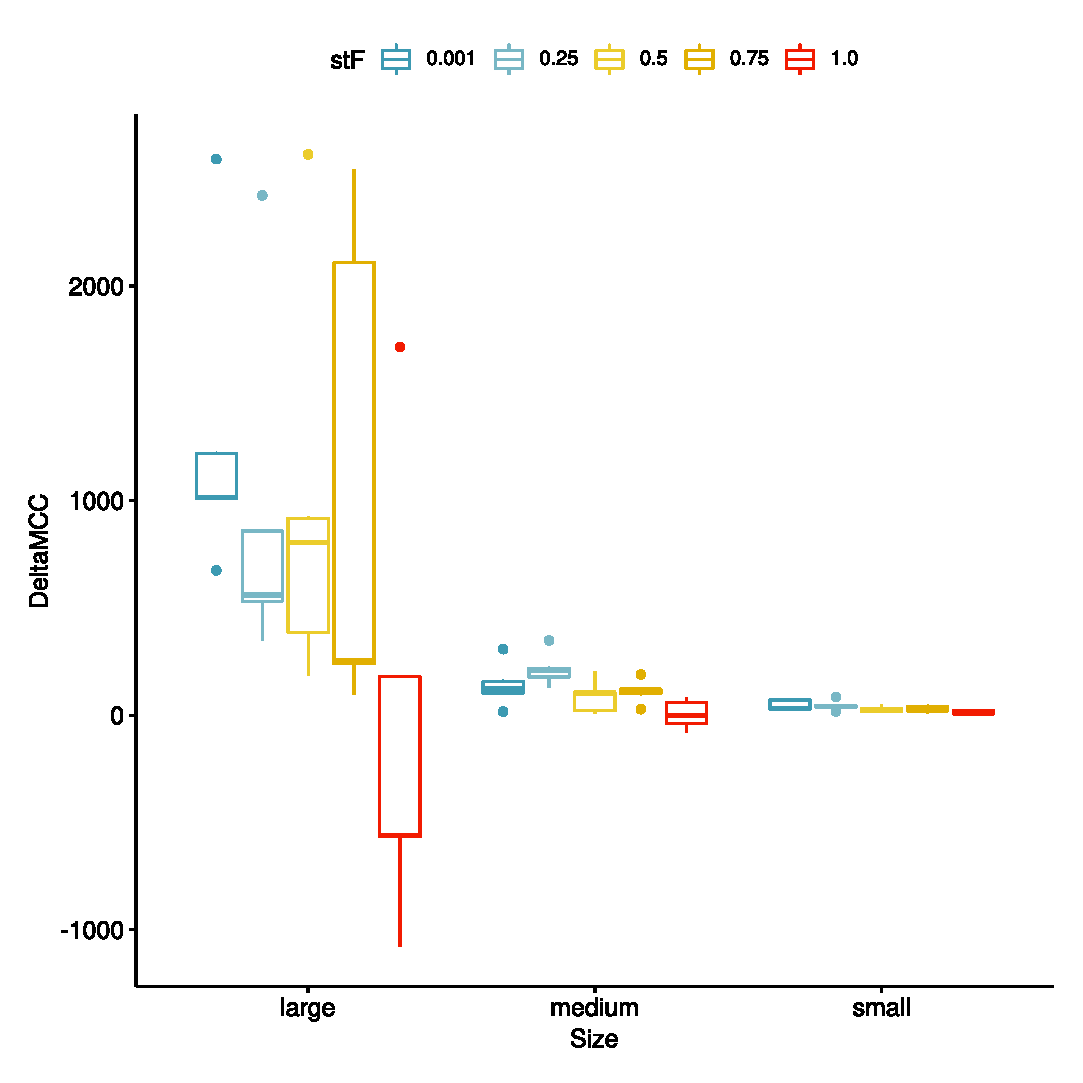
\includegraphics[width=.49\textwidth]{images/paper/results/mcc_box.eps}
 }
\caption{Summary results from the data sets.}
\end{figure}

As we can see from the Residuals vs. Fitted plot, depicted in Figure \ref{fig:ex1_qqplots}, the homogeneity of variance assumption is not met. To validate this observation we used Levene's Test. In this test, the null-hypotheses ($H_0$) asserts that the variance is equally distributed. As expected, from our observations of the Residuals vs Fitted Values plot, the test produced an F-value of 19.962 and a p-value of 1.267e-07 indicating that we should reject the null hypothesis that there is a homogeneity of variance.

The Normal Q-Q plot, depicted in Figure \ref{fig:ex1_qqplots}, indicates that the normality of the residuals assumption is also violated. To validate this observation we conducted both an Anderson-Darling GOF test against the Normal distribution. In this test the null-hypothesis ($H_0$) is that the empirical distribution is Normal. The results show that the A statistic has a value of 6.8257 and an associated p-value of < 2.2e-16 which indicates that we can reject the null-hypothesis. These results confirm our initial observation that the results are not normally distributed.

\begin{figure}[tb]
 \centering
 \subfloat[$\Delta HAL$ experiment interaction plot.]{
   \label{fig:ex1_interaction}
   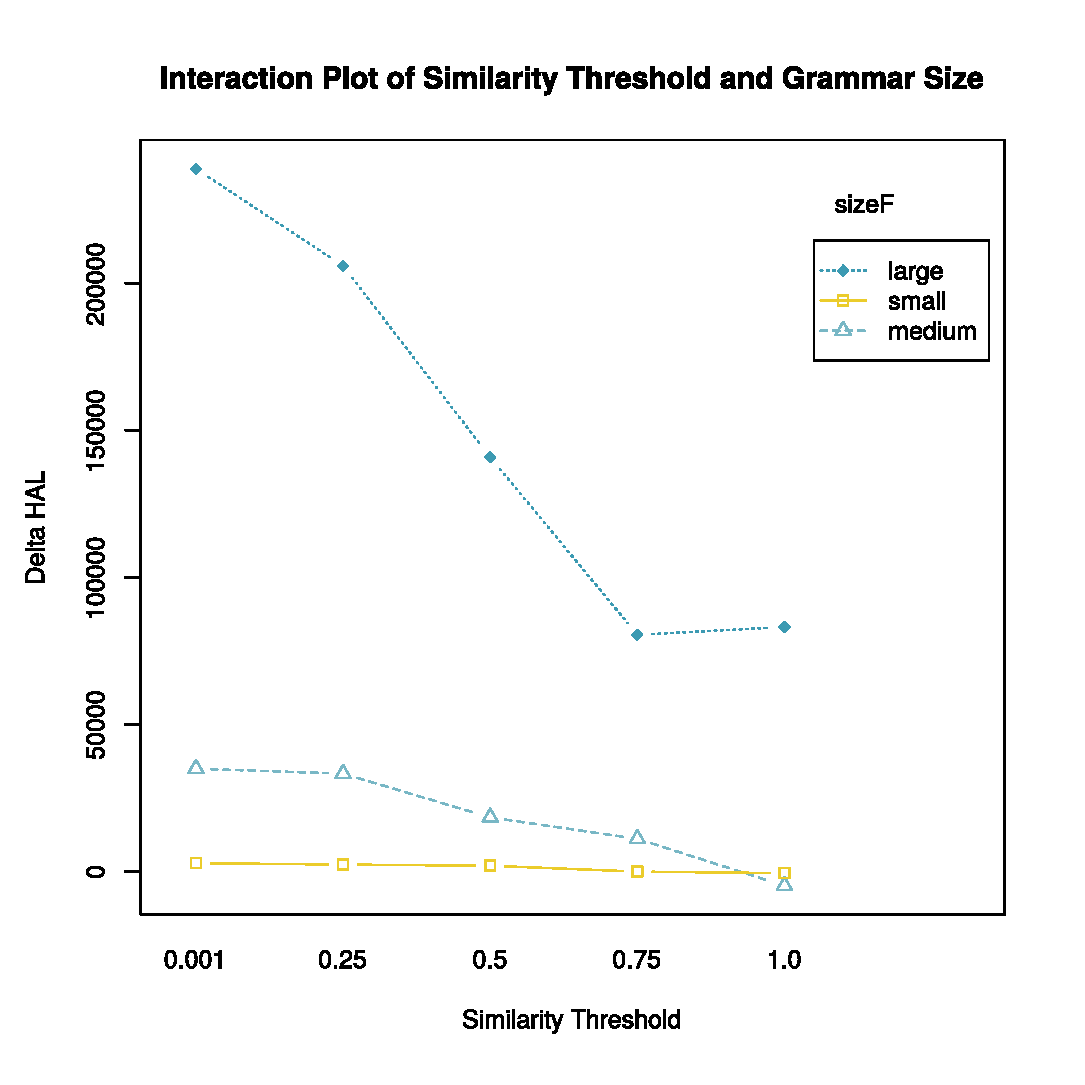
\includegraphics[width=.49\textwidth]{images/paper/results/ex1_interaction.eps}
 }
 \subfloat[$\Delta MCC$ experiment interaction plot.]{
   \label{fig:ex2_interaction}
   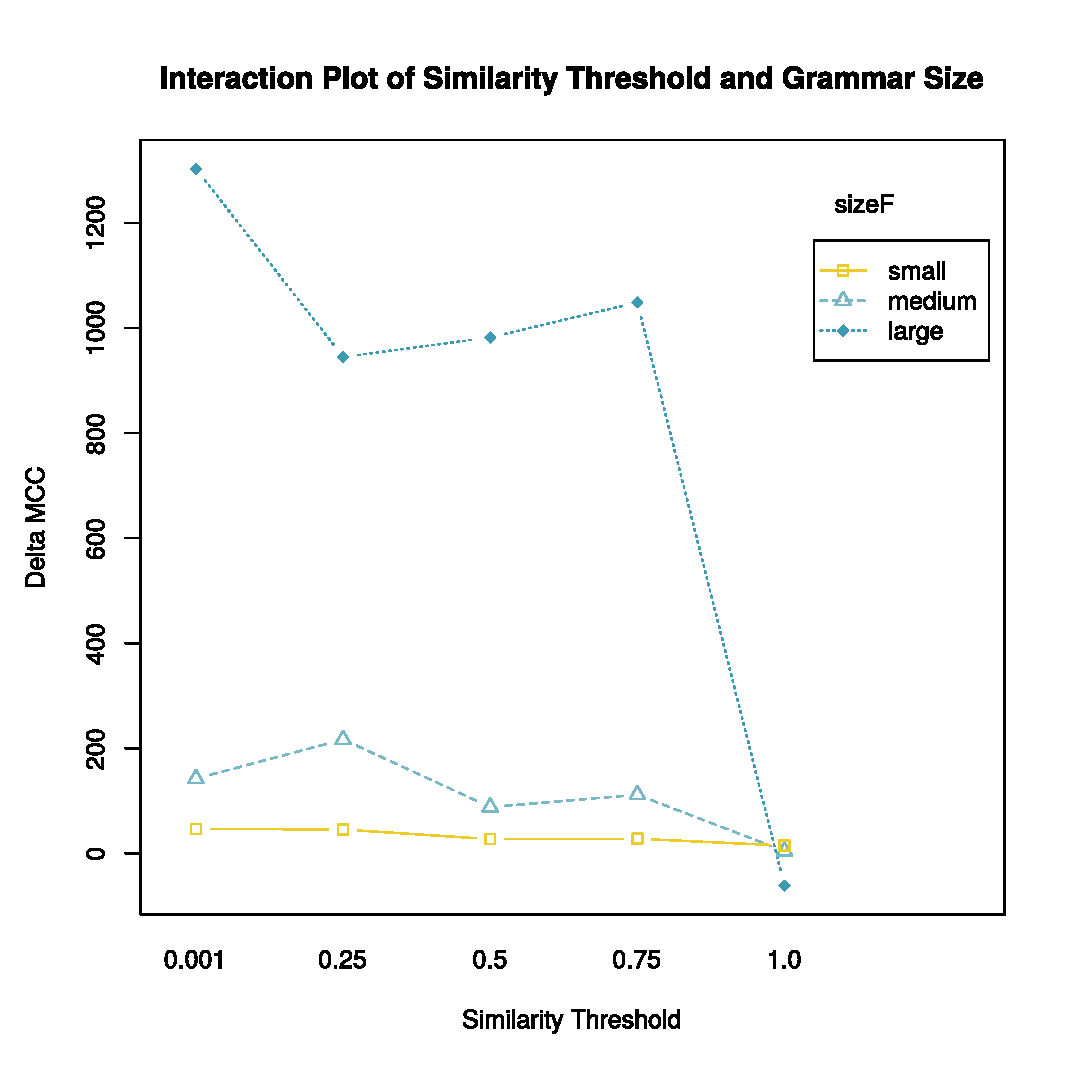
\includegraphics[width=.49\textwidth]{images/paper/results/ex2_interaction.eps}
 }
 \caption{Interaction plots for both (a) $\Delta HAL$ and (b) $\Delta MCC$ experiments.}
\end{figure}

The interaction plot, depicted in Figure \ref{fig:ex1_interaction}, indicates that their is an interaction between the small and medium levels as the similarity threshold changes from 0.75 to 1.0.


As we can see from the Residuals vs. Fitted plot, depicted in Figure \ref{fig:ex2_qqplots}, the homogeneity of variance assumption is not met. To validate this observation we used Levene's Test. In this test, the null-hypotheses ($H_0$) asserts that the variance is equally distributed. As expected, from our observations of the Residuals vs Fitted Values plot, the test produced an F-value of 29.856 and a p-value of 3.61e-10 indicating that we should reject the null hypothesis that there is a homogeneity of variance.

The Normal Q-Q plot, depicted in Figure \ref{fig:ex2_qqplots}, indicates that the normality of the residuals assumption is also violated. To validate this observation we conducted both an Anderson-Darling GOF test against the Normal distribution. In this test the null-hypothesis ($H_0$) is that the empirical distribution is Normal. The results show the A statistic has a value of 9.9558 and an associated p-value of < 2.2e-16 which indicates that we can reject the null-hypothesis. These results confirm our initial observation that the results are not normally distributed.


The interaction plot, depicted in Figure \ref{fig:ex2_interaction}, indicates that their is an interaction between the small and medium levels as the similarity threshold changes from 0.75 to 1.0.

\subsection{Hypothesis Testing}

This subsection details the results of the $\Delta HAL$ experiment and $\Delta MCC$ experiment. In both cases we initially executed a sample size analysis to determine the number of replications to execute to achieve a power level of .95. The results of this analysis indicate the need to execute a total of 5 replications of each experiment.

\subsubsection{$\Delta HAL$ Experiment}

We conducted an experiment using a factorial design based on the levels of the factors size and similarity threshold. Our goal was to determine if the algorithm when applied had an effect on the change in Halstead Effort for the combined grammars, as measured by $\Delta HAL$. Because of the violations to the assumptions of ANOVA, we were opted to utilize non-parametric methods in our analysis. The initial analysis utilize a permutation F-test approach to evaluate if there is any difference among factor levels. The results was an F-Value of XXXX and a p-value of XXXX indicating that we could reject $H_{1,0}$. We also note that the interaction indicated in Figure \ref{fig:ex1_interaction} was shown to be significant with an F-Value of XXXX and a p-value of XXXXX.

We were interested in determining if there was any difference between the control level (1.0) and other levels of the similarity threshold. To evaluate this we used Steel's multiple comparison against a control. The results of this test indicated for each level that there was a significant difference and that each level the mean $\Delta HAL$ was lower than that of the control value.

Finally, we were interested in evaluating the selected levels of the similarity threshold (excluding control) and if there was an implied order (that is there is a decreasing order to the change in $\Delta HAL$) as the level value is lowered in the similarity threshold. To evaluate this we used Jonchkheere's trend test for ordered differences among classes, which yields a JT statistic value of XXX and a p-value of XXXX, when executed using 10000 permutations. This indicates that we can reject $H_{3,0}$ that there is no \textit{a priori} ordering among levels of similarity threshold on median $\Delta HAL$.

\subsubsection{$\Delta MCC$ Experiment}

We conducted an experiment using a factorial design based on the levels of the factors size and similarity threshold. Our goal was to determine if the algorithm when applied had an effect on the change in Complexity for the combined grammars, as measured by $\Delta MCC$. Because of the violations to the assumptions of ANOVA, we were opted to utilize non-parametric methods in our analysis. The initial analysis utilize a permutation F-test approach to evaluate if there is any difference among factor levels. The results was an F-Value of XXXX and a p-value of XXXX indicating that we could reject $H_{1,0}$. We also note that the interaction indicated in Figure \ref{fig:ex2_interaction} was shown to be significant with an F-Value of XXXX and a p-value of XXXXX.

We were interested in determining if there was any difference between the control level (1.0) and other levels of the similarity threshold. To evaluate this we used Steel's multiple comparison against a control. The results of this test indicated for each level that there was a significant difference and that each level the mean $\Delta MCC$ was lower than that of the control value.

Finally, we were interested in evaluating the selected levels of the similarity threshold (excluding control) and if there was an implied order (that is there is a decreasing order to the change in $\Delta MCC$) as the level value is lowered in the similarity threshold. To evaluate this we used Jonchkheere's trend test for ordered differences among classes, which yields a JT statistic value of 767 and a p-value of 6e-04, when executed using 10000 permutations. Indicating that we can reject $H_{3,0}$ that there is no \textit{a priori} ordering among levels of similarity threshold on median $\Delta MCC$.

\section{Experiment 3: Evaluating Islandization}

\subsection{Descriptive Statistics}

\subsection{Hypothesis Testing}

\section{Experiment 4: Evaluating Tolerization}

\subsection{Descriptive Statistics}

\subsection{Hypothesis Testing}

\section{Experiment 5: Evaluating Bounding the Seas}

\subsection{Descriptive Statistics}

\subsection{Hypothesis Testing}

\section{Experiment 6: Evaluating Bridgization}

\subsection{Descriptive Statistics}

\subsection{Hypothesis Testing}

\chapter{Analysis and Interpretation}

The results indicate that the proposed merge process embodied in our algorithm reduces the Halstead Effort and McCabe Cyclomatic Complexity of a combined grammar at each threshold below the control threshold, regardless of size. The results also indicate  there is a increasing order to the amount of change in Halstead effort and Cyclomatic Complexity caused by the algorithm as the similarity threshold decreases. This implies that smaller values of the similarity threshold produce better results.

Since this was a randomized experiment, one may infer that the difference in Halstead Effort and McCabe Cyclomatic Complexity was caused by the difference in similarity threshold. Because the subjects were selected randomly from the population of Antlr grammars, we can extend this inference to that population. But, extending this inference to the population of grammars as a whole is speculative at best. This deficiency, however, is minor; the causal relationship is strong even though it applies only to Antlr grammars.


\chapter{Threats to Validity}

\section{Experiment 1: Evaluating Normalization}

\section{Experiment 2: Evaluating Merging}

We focused on threats to the conclusion, construct, internal, and external validity as detailed by Wohlin et al. \cite{wohlin_experimentation_2012}. We have identified no threats to the conclusion and construct validity of this study. But, there is a threat to the internal validity of this study. Specifically, we selected grammars from the ANTLR repository which limits the grammars available as well as the formats in which they are implemented. This is a threat due to the under-representation of the domain. Additionally, since we restrict our internal representations to BNF and Antlr4 and do not include the ability to utilize TXL, SDF or other grammar formats, there is a threat to external validity.

\section{Experiment 3: Evaluating Islandiation}

\section{Experiment 4: Evaluating Tolerization}

\section{Experiment 5: Evaluating Bounding the Seas}

\section{Experiment 6: Evaluating Bridgization}

\chapter{Conclusions and Future Work}

In this paper we have developed an algorithmic approach to merging programming language grammars together. The goal of this approach is to facilitate the automatic creation of Island Grammars for use in the development of multi-lingual software analysis tools. We evaluate this approach through two experiments on combined grammars selected from the Antlr grammar repository. These experiments evaluated the effects of this approach on changes to Halstead Effort and McCabe Cyclomatic Complexity of the grammar pairs as they are merged. The results show that the merging approach reduces the Halstead Effort and Cyclomatic Complexity when taking both grammar size and similarity threshold into consideration.

The results of this study are promising and present a potentially fruitful avenue towards the development of an automated approach to Island Grammar generation. Island Grammars have been shown to be an extremely useful approach for the development of multi-lingual analysis tools, but can be time-consuming to develop.

Immediate avenues for future work are as follows. We intended to conduct further studies to improve the results herein by expanding the study to grammars selected from the GrammarZoo \cite{zaytsev_grammar_2015} collection. As part of this we intend to extend the capabilities of this approach to incorporate TXL and SDF grammars which will also reduce threats to validity identified in Section \ref{sec:threats}. The results herein indicate the promise of this approach and we intend to integrate it with ongoing work to develop tools which will support the automated construction of island grammars for use in static analysis and quality measurement of software systems.

\bibliographystyle{IEEEtran}
\bibliography{references.bib}

\end{document}
